\begin{figure}[p]
{\figurefontsize
\centering
\begingroup%
  \makeatletter%
  \providecommand\color[2][]{%
    \errmessage{(Inkscape) Color is used for the text in Inkscape, but the package 'color.sty' is not loaded}%
    \renewcommand\color[2][]{}%
  }%
  \providecommand\transparent[1]{%
    \errmessage{(Inkscape) Transparency is used (non-zero) for the text in Inkscape, but the package 'transparent.sty' is not loaded}%
    \renewcommand\transparent[1]{}%
  }%
  \providecommand\rotatebox[2]{#2}%
  \newcommand*\fsize{\dimexpr\f@size pt\relax}%
  \newcommand*\lineheight[1]{\fontsize{\fsize}{#1\fsize}\selectfont}%
  \ifx\svgwidth\undefined%
    \setlength{\unitlength}{206.33378948bp}%
    \ifx\svgscale\undefined%
      \relax%
    \else%
      \setlength{\unitlength}{\unitlength * \real{\svgscale}}%
    \fi%
  \else%
    \setlength{\unitlength}{\svgwidth}%
  \fi%
  \global\let\svgwidth\undefined%
  \global\let\svgscale\undefined%
  \makeatother%
  \begin{picture}(1,0.92701271)%
    \lineheight{1}%
    \setlength\tabcolsep{0pt}%
    \put(0,0){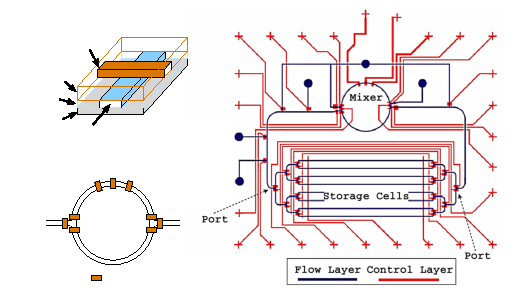
\includegraphics[width=\unitlength,page=1]{valve_mixer_storage_own_mixer.pdf}}%
    \put(0.50184519,0.0088474){\color[rgb]{0,0,0}\makebox(0,0)[lt]{\lineheight{0}\smash{\begin{tabular}[t]{l}(c) \end{tabular}}}}%
    \put(0.21834563,0.55772891){\color[rgb]{0,0,0}\makebox(0,0)[lt]{\lineheight{0}\smash{\begin{tabular}[t]{l}(a) \end{tabular}}}}%
    \put(0.81478559,0.55606846){\color[rgb]{0,0,0}\makebox(0,0)[lt]{\lineheight{0}\smash{\begin{tabular}[t]{l}(b) \end{tabular}}}}%
    \put(0.82769538,0.6186672){\color[rgb]{0,0,0}\makebox(0,0)[lt]{\lineheight{0}\smash{\begin{tabular}[t]{l}valve\end{tabular}}}}%
    \put(0,0){\includegraphics[width=\unitlength,page=2]{valve_mixer_storage_own_mixer.pdf}}%
    \put(0.8352133,0.75364771){\color[rgb]{0,0,0}\makebox(0,0)[t]{\lineheight{0}\smash{\begin{tabular}[t]{c}mixer\end{tabular}}}}%
    \put(0.83800497,0.90136719){\color[rgb]{0,0,0}\makebox(0,0)[t]{\lineheight{0}\smash{\begin{tabular}[t]{c}peristalsis valves\end{tabular}}}}%
    \put(0,0){\includegraphics[width=\unitlength,page=3]{valve_mixer_storage_own_mixer.pdf}}%
    \put(0.09749112,0.78640528){\color[rgb]{0,0,0}\makebox(0,0)[rt]{\lineheight{0}\smash{\begin{tabular}[t]{r}control layer\end{tabular}}}}%
    \put(0.56595478,0.69987763){\color[rgb]{0,0,0}\makebox(0,0)[rt]{\lineheight{0}\smash{\begin{tabular}[t]{r}flow layer\end{tabular}}}}%
    \put(0.16380156,0.63300966){\color[rgb]{0,0,0}\makebox(0,0)[t]{\lineheight{0}\smash{\begin{tabular}[t]{c}flow\end{tabular}}}}%
    \put(0.08243246,0.64072703){\color[rgb]{0,0,0}\makebox(0,0)[rt]{\lineheight{0}\smash{\begin{tabular}[t]{r}substrate\end{tabular}}}}%
    \put(0.16134671,0.59549907){\color[rgb]{0,0,0}\makebox(0,0)[t]{\lineheight{0}\smash{\begin{tabular}[t]{c}channel\end{tabular}}}}%
    \put(0,0){\includegraphics[width=\unitlength,page=4]{valve_mixer_storage_own_mixer.pdf}}%
    \put(0.51286637,0.82103479){\color[rgb]{0,0,0}\makebox(0,0)[t]{\lineheight{0}\smash{\begin{tabular}[t]{c}control\end{tabular}}}}%
    \put(0.51286637,0.78168834){\color[rgb]{0,0,0}\makebox(0,0)[t]{\lineheight{0}\smash{\begin{tabular}[t]{c}channel\end{tabular}}}}%
  \end{picture}%
\endgroup%
\label{fig:valve_mixer_storage}
}
\end{figure}
	\clearpage
\begin{figure}[p]
{\figurefontsize
\centering
\begingroup%
  \makeatletter%
  \providecommand\color[2][]{%
    \errmessage{(Inkscape) Color is used for the text in Inkscape, but the package 'color.sty' is not loaded}%
    \renewcommand\color[2][]{}%
  }%
  \providecommand\transparent[1]{%
    \errmessage{(Inkscape) Transparency is used (non-zero) for the text in Inkscape, but the package 'transparent.sty' is not loaded}%
    \renewcommand\transparent[1]{}%
  }%
  \providecommand\rotatebox[2]{#2}%
  \newcommand*\fsize{\dimexpr\f@size pt\relax}%
  \newcommand*\lineheight[1]{\fontsize{\fsize}{#1\fsize}\selectfont}%
  \ifx\svgwidth\undefined%
    \setlength{\unitlength}{253.05725098bp}%
    \ifx\svgscale\undefined%
      \relax%
    \else%
      \setlength{\unitlength}{\unitlength * \real{\svgscale}}%
    \fi%
  \else%
    \setlength{\unitlength}{\svgwidth}%
  \fi%
  \global\let\svgwidth\undefined%
  \global\let\svgscale\undefined%
  \makeatother%
  \begin{picture}(1,0.4460739)%
    \lineheight{1}%
    \setlength\tabcolsep{0pt}%
    \put(0.82960669,0.00534793){\color[rgb]{0,0,0}\makebox(0,0)[t]{\lineheight{0}\smash{\begin{tabular}[t]{c}(c)\end{tabular}}}}%
    \put(0.17206719,0.00534793){\color[rgb]{0,0,0}\makebox(0,0)[t]{\lineheight{0}\smash{\begin{tabular}[t]{c}(a)\end{tabular}}}}%
    \put(0.50153204,0.00534793){\color[rgb]{0,0,0}\makebox(0,0)[t]{\lineheight{0}\smash{\begin{tabular}[t]{c}(b)\end{tabular}}}}%
    \put(0,0){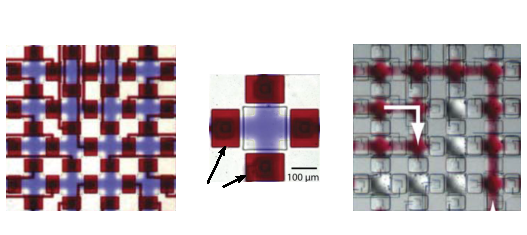
\includegraphics[width=\unitlength,page=1]{archi.pdf}}%
    \put(0.40181094,0.07336126){\color[rgb]{0,0,0}\makebox(0,0)[t]{\lineheight{1.25}\smash{\begin{tabular}[t]{c}valves\end{tabular}}}}%
    \put(0,0){\includegraphics[width=\unitlength,page=2]{archi.pdf}}%
    \put(0.5682774,0.36219924){\color[rgb]{0,0,0}\makebox(0,0)[t]{\lineheight{0}\smash{\begin{tabular}[t]{c}channel\end{tabular}}}}%
    \put(0,0){\includegraphics[width=\unitlength,page=3]{archi.pdf}}%
    \put(0.16168071,0.42865935){\color[rgb]{0,0,0}\makebox(0,0)[t]{\lineheight{0}\smash{\begin{tabular}[t]{c}control\end{tabular}}}}%
    \put(0.16168071,0.40111931){\color[rgb]{0,0,0}\makebox(0,0)[t]{\lineheight{0}\smash{\begin{tabular}[t]{c}channel\end{tabular}}}}%
    \put(0,0){\includegraphics[width=\unitlength,page=4]{archi.pdf}}%
    \put(0.36786319,0.42865935){\color[rgb]{0,0,0}\makebox(0,0)[t]{\lineheight{0}\smash{\begin{tabular}[t]{c}channel\end{tabular}}}}%
    \put(0.36797696,0.40111931){\color[rgb]{0,0,0}\makebox(0,0)[t]{\lineheight{0}\smash{\begin{tabular}[t]{c}wall\end{tabular}}}}%
    \put(0.5678822,0.38968332){\color[rgb]{0,0,0}\makebox(0,0)[t]{\lineheight{0}\smash{\begin{tabular}[t]{c}flow\end{tabular}}}}%
    \put(0.56778639,0.33379743){\color[rgb]{0,0,0}\makebox(0,0)[t]{\lineheight{0}\smash{\begin{tabular}[t]{c}(cell)\end{tabular}}}}%
  \end{picture}%
\endgroup%
\label{fig:archi}
}
\end{figure}
	\clearpage
\begin{figure}[p]
{\figurefontsize
\centering
\begingroup%
  \makeatletter%
  \providecommand\color[2][]{%
    \errmessage{(Inkscape) Color is used for the text in Inkscape, but the package 'color.sty' is not loaded}%
    \renewcommand\color[2][]{}%
  }%
  \providecommand\transparent[1]{%
    \errmessage{(Inkscape) Transparency is used (non-zero) for the text in Inkscape, but the package 'transparent.sty' is not loaded}%
    \renewcommand\transparent[1]{}%
  }%
  \providecommand\rotatebox[2]{#2}%
  \newcommand*\fsize{\dimexpr\f@size pt\relax}%
  \newcommand*\lineheight[1]{\fontsize{\fsize}{#1\fsize}\selectfont}%
  \ifx\svgwidth\undefined%
    \setlength{\unitlength}{223.41824396bp}%
    \ifx\svgscale\undefined%
      \relax%
    \else%
      \setlength{\unitlength}{\unitlength * \real{\svgscale}}%
    \fi%
  \else%
    \setlength{\unitlength}{\svgwidth}%
  \fi%
  \global\let\svgwidth\undefined%
  \global\let\svgscale\undefined%
  \makeatother%
  \begin{picture}(1,1.06660424)%
    \lineheight{1}%
    \setlength\tabcolsep{0pt}%
    \put(0.7342614,0.62280321){\color[rgb]{0,0,0}\makebox(0,0)[t]{\lineheight{0}\smash{\begin{tabular}[t]{c}(b)\end{tabular}}}}%
    \put(0.47722094,1.02888716){\color[rgb]{0,0,0}\makebox(0,0)[lt]{\lineheight{0}\smash{\begin{tabular}[t]{l}: closed / wall valves\end{tabular}}}}%
    \put(0,0){
\includegraphics[width=\unitlength,page=1]{dynamic_devices.pdf}}%
    \put(0.17288269,0.84756997){\color[rgb]{0,0,0}\makebox(0,0)[t]{\lineheight{0}\smash{\begin{tabular}[t]{c} \end{tabular}}}}%
    \put(0.10521609,0.53617861){\color[rgb]{0,0,0}\makebox(0,0)[t]{\lineheight{0}\smash{\begin{tabular}[t]{c}(a)\end{tabular}}}}%
    \put(0,0){
\includegraphics[width=\unitlength,page=2]{dynamic_devices.pdf}}%
    \put(0.47722094,0.95302425){\color[rgb]{0,0,0}\makebox(0,0)[lt]{\lineheight{0}\smash{\begin{tabular}[t]{l}: peristalsis valves\end{tabular}}}}%
    \put(0,0){
\includegraphics[width=\unitlength,page=3]{dynamic_devices.pdf}}%
    \put(0.03357004,1.03151406){\color[rgb]{0,0,0}\makebox(0,0)[t]{\lineheight{0}\smash{\begin{tabular}[t]{c}valves\end{tabular}}}}%
    \put(0,0){
\includegraphics[width=\unitlength,page=4]{dynamic_devices.pdf}}%
    \put(0.16852922,1.03185746){\color[rgb]{0,0,0}\makebox(0,0)[t]{\lineheight{1.25}\smash{\begin{tabular}[t]{c}channel\end{tabular}}}}%
    \put(0.19676309,0.00810385){\color[rgb]{0,0,0}\makebox(0,0)[t]{\lineheight{0}\smash{\begin{tabular}[t]{c}(c)\end{tabular}}}}%
    \put(0.71873631,0.00810385){\color[rgb]{0,0,0}\makebox(0,0)[t]{\lineheight{0}\smash{\begin{tabular}[t]{c}(d)\end{tabular}}}}%
    \put(0,0){
\includegraphics[width=\unitlength,page=5]{dynamic_devices.pdf}}%
    \put(0.5820626,0.56096611){\color[rgb]{0,0,0}\makebox(0,0)[t]{\lineheight{1.25}\smash{\begin{tabular}[t]{c}no valve\end{tabular}}}}%
    \put(0.81906841,0.51804577){\color[rgb]{0,0,0}\makebox(0,0)[t]{\lineheight{0}\smash{\begin{tabular}[t]{c}always-closed valves\end{tabular}}}}%
    \put(0,0){
\includegraphics[width=\unitlength,page=6]{dynamic_devices.pdf}}%
    \put(0.55367855,0.04238681){\color[rgb]{0,0,0}\makebox(0,0)[t]{\lineheight{1.25}\smash{\begin{tabular}[t]{c}1\end{tabular}}}}%
    \put(0.59889592,0.04227309){\color[rgb]{0,0,0}\makebox(0,0)[t]{\lineheight{1.25}\smash{\begin{tabular}[t]{c}2\end{tabular}}}}%
    \put(0.64436173,0.04240873){\color[rgb]{0,0,0}\makebox(0,0)[t]{\lineheight{1.25}\smash{\begin{tabular}[t]{c}3\end{tabular}}}}%
    \put(0.68991328,0.04240873){\color[rgb]{0,0,0}\makebox(0,0)[t]{\lineheight{1.25}\smash{\begin{tabular}[t]{c}4\end{tabular}}}}%
    \put(0.73461381,0.04254416){\color[rgb]{0,0,0}\makebox(0,0)[t]{\lineheight{1.25}\smash{\begin{tabular}[t]{c}5\end{tabular}}}}%
    \put(0.78008228,0.04242184){\color[rgb]{0,0,0}\makebox(0,0)[t]{\lineheight{1.25}\smash{\begin{tabular}[t]{c}6\end{tabular}}}}%
    \put(0.82540477,0.04240873){\color[rgb]{0,0,0}\makebox(0,0)[t]{\lineheight{1.25}\smash{\begin{tabular}[t]{c}7\end{tabular}}}}%
    \put(0.87091247,0.04240873){\color[rgb]{0,0,0}\makebox(0,0)[t]{\lineheight{1.25}\smash{\begin{tabular}[t]{c}8\end{tabular}}}}%
    \put(0.91598909,0.04240422){\color[rgb]{0,0,0}\makebox(0,0)[t]{\lineheight{1.25}\smash{\begin{tabular}[t]{c}9\end{tabular}}}}%
    \put(0.48590842,0.10546882){\color[rgb]{0,0,0}\makebox(0,0)[t]{\lineheight{1.25}\smash{\begin{tabular}[t]{c}1\end{tabular}}}}%
    \put(0.48604826,0.15036718){\color[rgb]{0,0,0}\makebox(0,0)[t]{\lineheight{1.25}\smash{\begin{tabular}[t]{c}2\end{tabular}}}}%
    \put(0.48611382,0.19590276){\color[rgb]{0,0,0}\makebox(0,0)[t]{\lineheight{1.25}\smash{\begin{tabular}[t]{c}3\end{tabular}}}}%
    \put(0.48626677,0.24130105){\color[rgb]{0,0,0}\makebox(0,0)[t]{\lineheight{1.25}\smash{\begin{tabular}[t]{c}4\end{tabular}}}}%
    \put(0.4859871,0.28670487){\color[rgb]{0,0,0}\makebox(0,0)[t]{\lineheight{1.25}\smash{\begin{tabular}[t]{c}5\end{tabular}}}}%
    \put(0.48605696,0.3300979){\color[rgb]{0,0,0}\makebox(0,0)[t]{\lineheight{1.25}\smash{\begin{tabular}[t]{c}6\end{tabular}}}}%
    \put(0.48606137,0.37548513){\color[rgb]{0,0,0}\makebox(0,0)[t]{\lineheight{1.25}\smash{\begin{tabular}[t]{c}7\end{tabular}}}}%
    \put(0.48617068,0.42088322){\color[rgb]{0,0,0}\makebox(0,0)[t]{\lineheight{1.25}\smash{\begin{tabular}[t]{c}8\end{tabular}}}}%
    \put(0.48626677,0.46614751){\color[rgb]{0,0,0}\makebox(0,0)[t]{\lineheight{1.25}\smash{\begin{tabular}[t]{c}9\end{tabular}}}}%
  \end{picture}%
\endgroup%
\label{fig:dynamic_devices}
}
\end{figure}
	\clearpage
\begin{figure}[p]
{\figurefontsize
\centering
\begingroup%
  \makeatletter%
  \providecommand\color[2][]{%
    \errmessage{(Inkscape) Color is used for the text in Inkscape, but the package 'color.sty' is not loaded}%
    \renewcommand\color[2][]{}%
  }%
  \providecommand\transparent[1]{%
    \errmessage{(Inkscape) Transparency is used (non-zero) for the text in Inkscape, but the package 'transparent.sty' is not loaded}%
    \renewcommand\transparent[1]{}%
  }%
  \providecommand\rotatebox[2]{#2}%
  \newcommand*\fsize{\dimexpr\f@size pt\relax}%
  \newcommand*\lineheight[1]{\fontsize{\fsize}{#1\fsize}\selectfont}%
  \ifx\svgwidth\undefined%
    \setlength{\unitlength}{225.61093897bp}%
    \ifx\svgscale\undefined%
      \relax%
    \else%
      \setlength{\unitlength}{\unitlength * \real{\svgscale}}%
    \fi%
  \else%
    \setlength{\unitlength}{\svgwidth}%
  \fi%
  \global\let\svgwidth\undefined%
  \global\let\svgscale\undefined%
  \makeatother%
  \begin{picture}(1,0.9140426)%
    \lineheight{1}%
    \setlength\tabcolsep{0pt}%
    \put(0,0){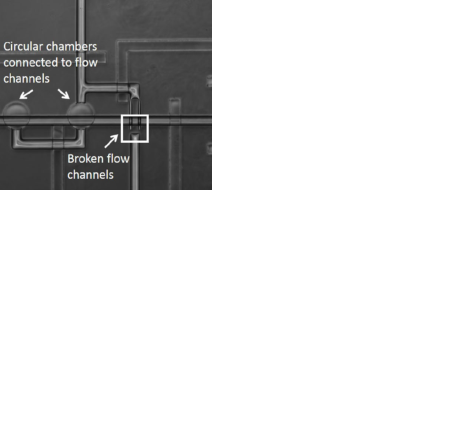
\includegraphics[width=\unitlength,page=1]{defects.pdf}}%
    \put(0.21563204,0.47229537){\color[rgb]{0,0,0}\makebox(0,0)[t]{\lineheight{0}\smash{\begin{tabular}[t]{c}(a)\end{tabular}}}}%
    \put(0,0){\includegraphics[width=\unitlength,page=2]{defects.pdf}}%
    \put(0.75841029,0.47208699){\color[rgb]{0,0,0}\makebox(0,0)[t]{\lineheight{0}\smash{\begin{tabular}[t]{c}(b)\end{tabular}}}}%
    \put(0,0){\includegraphics[width=\unitlength,page=3]{defects.pdf}}%
    \put(0.22785713,0.00657027){\color[rgb]{0,0,0}\makebox(0,0)[t]{\lineheight{0}\smash{\begin{tabular}[t]{c}(c)\end{tabular}}}}%
    \put(0,0){\includegraphics[width=\unitlength,page=4]{defects.pdf}}%
    \put(0.77838155,0.00636209){\color[rgb]{0,0,0}\makebox(0,0)[t]{\lineheight{0}\smash{\begin{tabular}[t]{c}(d)\end{tabular}}}}%
  \end{picture}%
\endgroup%
\label{fig:defects}
}
\end{figure}
	\clearpage
\begin{figure}[p]
{\figurefontsize
\centering
\begingroup%
  \makeatletter%
  \providecommand\color[2][]{%
    \errmessage{(Inkscape) Color is used for the text in Inkscape, but the package 'color.sty' is not loaded}%
    \renewcommand\color[2][]{}%
  }%
  \providecommand\transparent[1]{%
    \errmessage{(Inkscape) Transparency is used (non-zero) for the text in Inkscape, but the package 'transparent.sty' is not loaded}%
    \renewcommand\transparent[1]{}%
  }%
  \providecommand\rotatebox[2]{#2}%
  \newcommand*\fsize{\dimexpr\f@size pt\relax}%
  \newcommand*\lineheight[1]{\fontsize{\fsize}{#1\fsize}\selectfont}%
  \ifx\svgwidth\undefined%
    \setlength{\unitlength}{183.91088672bp}%
    \ifx\svgscale\undefined%
      \relax%
    \else%
      \setlength{\unitlength}{\unitlength * \real{\svgscale}}%
    \fi%
  \else%
    \setlength{\unitlength}{\svgwidth}%
  \fi%
  \global\let\svgwidth\undefined%
  \global\let\svgscale\undefined%
  \makeatother%
  \begin{picture}(1,0.7370509)%
    \lineheight{1}%
    \setlength\tabcolsep{0pt}%
    \put(0,0){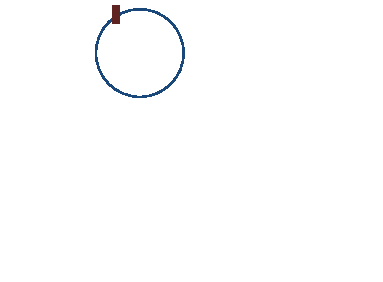
\includegraphics[width=\unitlength,page=1]{ref_test_biochip.pdf}}%
    \put(0.30335142,0.69036144){\color[rgb]{1,1,1}\makebox(0,0)[t]{\lineheight{0}\smash{\begin{tabular}[t]{c}c\end{tabular}}}}%
    \put(0,0){\includegraphics[width=\unitlength,page=2]{ref_test_biochip.pdf}}%
    \put(0.3625445,0.7063789){\color[rgb]{1,1,1}\makebox(0,0)[t]{\lineheight{0}\smash{\begin{tabular}[t]{c}d\end{tabular}}}}%
    \put(0,0){\includegraphics[width=\unitlength,page=3]{ref_test_biochip.pdf}}%
    \put(0.42173764,0.69036144){\color[rgb]{1,1,1}\makebox(0,0)[t]{\lineheight{0}\smash{\begin{tabular}[t]{c}e\end{tabular}}}}%
    \put(0,0){\includegraphics[width=\unitlength,page=4]{ref_test_biochip.pdf}}%
    \put(0.25655341,0.6224595){\color[rgb]{1,1,1}\makebox(0,0)[t]{\lineheight{0}\smash{\begin{tabular}[t]{c}b\end{tabular}}}}%
    \put(0,0){\includegraphics[width=\unitlength,page=5]{ref_test_biochip.pdf}}%
    \put(0.25655341,0.55573662){\color[rgb]{1,1,1}\makebox(0,0)[t]{\lineheight{0}\smash{\begin{tabular}[t]{c}g\end{tabular}}}}%
    \put(0,0){\includegraphics[width=\unitlength,page=6]{ref_test_biochip.pdf}}%
    \put(0.47553814,0.61831844){\color[rgb]{1,1,1}\makebox(0,0)[t]{\lineheight{0}\smash{\begin{tabular}[t]{c}f\end{tabular}}}}%
    \put(0,0){\includegraphics[width=\unitlength,page=7]{ref_test_biochip.pdf}}%
    \put(0.47553814,0.54628108){\color[rgb]{1,1,1}\makebox(0,0)[t]{\lineheight{0}\smash{\begin{tabular}[t]{c}h\end{tabular}}}}%
    \put(0,0){\includegraphics[width=\unitlength,page=8]{ref_test_biochip.pdf}}%
    \put(0.17281526,0.59033947){\color[rgb]{1,1,1}\makebox(0,0)[t]{\lineheight{0}\smash{\begin{tabular}[t]{c}a\end{tabular}}}}%
    \put(0,0){\includegraphics[width=\unitlength,page=9]{ref_test_biochip.pdf}}%
    \put(0.56100453,0.59033947){\color[rgb]{1,1,1}\makebox(0,0)[t]{\lineheight{0}\smash{\begin{tabular}[t]{c}i\end{tabular}}}}%
    \put(0,0){\includegraphics[width=\unitlength,page=10]{ref_test_biochip.pdf}}%
    \put(0.63822853,0.62623866){\color[rgb]{1,1,1}\makebox(0,0)[t]{\lineheight{0}\smash{\begin{tabular}[t]{c}j\end{tabular}}}}%
    \put(0,0){\includegraphics[width=\unitlength,page=11]{ref_test_biochip.pdf}}%
    \put(0.63822853,0.55137869){\color[rgb]{1,1,1}\makebox(0,0)[t]{\lineheight{0}\smash{\begin{tabular}[t]{c}k\end{tabular}}}}%
    \put(0,0){\includegraphics[width=\unitlength,page=12]{ref_test_biochip.pdf}}%
    \put(-0.00158789,0.69234335){\color[rgb]{0,0,0}\makebox(0,0)[lt]{\lineheight{0}\smash{\begin{tabular}[t]{l}pressure \end{tabular}}}}%
    \put(-0.0003241,0.6536972){\color[rgb]{0,0,0}\makebox(0,0)[lt]{\lineheight{0}\smash{\begin{tabular}[t]{l}source\end{tabular}}}}%
    \put(0,0){\includegraphics[width=\unitlength,page=13]{ref_test_biochip.pdf}}%
    \put(0.76060006,0.51949584){\color[rgb]{1,1,1}\makebox(0,0)[t]{\lineheight{0}\smash{\begin{tabular}[t]{c}$o_2$\end{tabular}}}}%
    \put(0.31587142,0.58773534){\color[rgb]{0,0,0}\makebox(0,0)[lt]{\lineheight{0}\smash{\begin{tabular}[t]{l}mixer\end{tabular}}}}%
    \put(0,0){\includegraphics[width=\unitlength,page=14]{ref_test_biochip.pdf}}%
    \put(0.84721895,0.60740523){\color[rgb]{0,0,0}\makebox(0,0)[lt]{\lineheight{0}\smash{\begin{tabular}[t]{l}pressure \end{tabular}}}}%
    \put(0.84848279,0.56875908){\color[rgb]{0,0,0}\makebox(0,0)[lt]{\lineheight{0}\smash{\begin{tabular}[t]{l}sensors\end{tabular}}}}%
    \put(0.76060006,0.66231447){\color[rgb]{1,1,1}\makebox(0,0)[t]{\lineheight{0}\smash{\begin{tabular}[t]{c}$o_1$\end{tabular}}}}%
    \put(0,0){\includegraphics[width=\unitlength,page=15]{ref_test_biochip.pdf}}%
    \put(0.06733809,0.17296396){\color[rgb]{0,0,0}\makebox(0,0)[t]{\lineheight{0}\smash{\begin{tabular}[t]{c}c\end{tabular}}}}%
    \put(0.06822243,0.25280406){\color[rgb]{0,0,0}\makebox(0,0)[t]{\lineheight{0}\smash{\begin{tabular}[t]{c}d\end{tabular}}}}%
    \put(0.06763522,0.23059059){\color[rgb]{0,0,0}\makebox(0,0)[t]{\lineheight{0}\smash{\begin{tabular}[t]{c}e\end{tabular}}}}%
    \put(0.06713295,0.28871955){\color[rgb]{0,0,0}\makebox(0,0)[t]{\lineheight{0}\smash{\begin{tabular}[t]{c}b\end{tabular}}}}%
    \put(0.06822243,0.14571584){\color[rgb]{0,0,0}\makebox(0,0)[t]{\lineheight{0}\smash{\begin{tabular}[t]{c}g\end{tabular}}}}%
    \put(0.06672966,0.20104251){\color[rgb]{0,0,0}\makebox(0,0)[t]{\lineheight{0}\smash{\begin{tabular}[t]{c}f\end{tabular}}}}%
    \put(0.06762109,0.10716967){\color[rgb]{0,0,0}\makebox(0,0)[t]{\lineheight{0}\smash{\begin{tabular}[t]{c}h\end{tabular}}}}%
    \put(0.0682083,0.35328228){\color[rgb]{0,0,0}\makebox(0,0)[t]{\lineheight{0}\smash{\begin{tabular}[t]{c}a\end{tabular}}}}%
    \put(0.06769185,0.32327734){\color[rgb]{0,0,0}\makebox(0,0)[t]{\lineheight{0}\smash{\begin{tabular}[t]{c}i\end{tabular}}}}%
    \put(0.06932609,0.38527859){\color[rgb]{0,0,0}\makebox(0,0)[t]{\lineheight{0}\smash{\begin{tabular}[t]{c}j\end{tabular}}}}%
    \put(0.06640422,0.07586297){\color[rgb]{0,0,0}\makebox(0,0)[t]{\lineheight{0}\smash{\begin{tabular}[t]{c}k\end{tabular}}}}%
    \put(0.86188074,0.09227412){\color[rgb]{0,0,0}\makebox(0,0)[t]{\lineheight{0}\smash{\begin{tabular}[t]{c}$o_2$\end{tabular}}}}%
    \put(0.86188074,0.37180712){\color[rgb]{0,0,0}\makebox(0,0)[t]{\lineheight{0}\smash{\begin{tabular}[t]{c}$o_1$\end{tabular}}}}%
    \put(0.40175302,0.43282083){\color[rgb]{0,0,0}\makebox(0,0)[lt]{\lineheight{0}\smash{\begin{tabular}[t]{l}(a)\end{tabular}}}}%
    \put(0.40139816,0.00664599){\color[rgb]{0,0,0}\makebox(0,0)[lt]{\lineheight{0}\smash{\begin{tabular}[t]{l}(b)\end{tabular}}}}%
    \put(0.63822853,0.62419961){\color[rgb]{1,1,1}\makebox(0,0)[t]{\lineheight{0}\smash{\begin{tabular}[t]{c}j\end{tabular}}}}%
  \end{picture}%
\endgroup%
\label{fig:classic_test}
}
\end{figure}
	\clearpage
\begin{figure}[p]
{\figurefontsize
\centering
\begingroup%
  \makeatletter%
  \providecommand\color[2][]{%
    \errmessage{(Inkscape) Color is used for the text in Inkscape, but the package 'color.sty' is not loaded}%
    \renewcommand\color[2][]{}%
  }%
  \providecommand\transparent[1]{%
    \errmessage{(Inkscape) Transparency is used (non-zero) for the text in Inkscape, but the package 'transparent.sty' is not loaded}%
    \renewcommand\transparent[1]{}%
  }%
  \providecommand\rotatebox[2]{#2}%
  \newcommand*\fsize{\dimexpr\f@size pt\relax}%
  \newcommand*\lineheight[1]{\fontsize{\fsize}{#1\fsize}\selectfont}%
  \ifx\svgwidth\undefined%
    \setlength{\unitlength}{257.44990564bp}%
    \ifx\svgscale\undefined%
      \relax%
    \else%
      \setlength{\unitlength}{\unitlength * \real{\svgscale}}%
    \fi%
  \else%
    \setlength{\unitlength}{\svgwidth}%
  \fi%
  \global\let\svgwidth\undefined%
  \global\let\svgscale\undefined%
  \makeatother%
  \begin{picture}(1,1.00777318)%
    \lineheight{1}%
    \setlength\tabcolsep{0pt}%
    \put(0,0){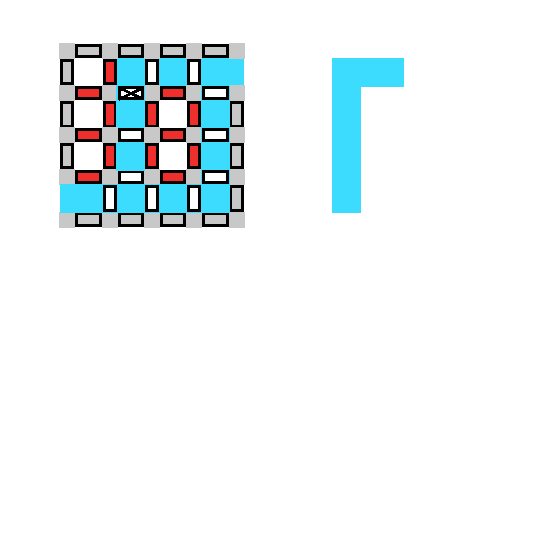
\includegraphics[width=\unitlength,page=1]{path_cutset.pdf}}%
    \put(0.52668259,0.88237203){\color[rgb]{0,0,0}\makebox(0,0)[t]{\lineheight{0}\smash{\begin{tabular}[t]{c}pressure\end{tabular}}}}%
    \put(0.52571585,0.85227999){\color[rgb]{0,0,0}\makebox(0,0)[t]{\lineheight{0}\smash{\begin{tabular}[t]{c}sensor\end{tabular}}}}%
    \put(0.00009957,0.64591962){\color[rgb]{0,0,0}\makebox(0,0)[lt]{\lineheight{0}\smash{\begin{tabular}[t]{l}pressure\end{tabular}}}}%
    \put(0.00444935,0.6152458){\color[rgb]{0,0,0}\makebox(0,0)[lt]{\lineheight{0}\smash{\begin{tabular}[t]{l}source\end{tabular}}}}%
    \put(0,0){\includegraphics[width=\unitlength,page=2]{path_cutset.pdf}}%
    \put(0.20421121,0.98754587){\color[rgb]{0,0,0}\makebox(0,0)[t]{\lineheight{0}\smash{\begin{tabular}[t]{c}valve under test\end{tabular}}}}%
    \put(0,0){\includegraphics[width=\unitlength,page=3]{path_cutset.pdf}}%
    \put(0.35809036,0.95820685){\color[rgb]{0,0,0}\makebox(0,0)[t]{\lineheight{0}\smash{\begin{tabular}[t]{c}path 1\end{tabular}}}}%
    \put(0.49969542,0.77663721){\color[rgb]{0,0,0}\makebox(0,0)[t]{\lineheight{0}\smash{\begin{tabular}[t]{c}path 2\end{tabular}}}}%
    \put(0,0){\includegraphics[width=\unitlength,page=4]{path_cutset.pdf}}%
    \put(0.74451826,0.95674883){\color[rgb]{0,0,0}\makebox(0,0)[t]{\lineheight{0}\smash{\begin{tabular}[t]{c}cut\end{tabular}}}}%
    \put(0,0){\includegraphics[width=\unitlength,page=5]{path_cutset.pdf}}%
    \put(0.28690947,0.49637158){\color[rgb]{0,0,0}\makebox(0,0)[t]{\lineheight{0}\smash{\begin{tabular}[t]{c}(a)\end{tabular}}}}%
    \put(0.76974034,0.49637158){\color[rgb]{0,0,0}\makebox(0,0)[t]{\lineheight{0}\smash{\begin{tabular}[t]{c}(b)\end{tabular}}}}%
    \put(0,0){\includegraphics[width=\unitlength,page=6]{path_cutset.pdf}}%
    \put(0.20828797,0.95820685){\color[rgb]{0,0,0}\makebox(0,0)[t]{\lineheight{0}\smash{\begin{tabular}[t]{c}(stuck-at-0)\end{tabular}}}}%
    \put(0,0){\includegraphics[width=\unitlength,page=7]{path_cutset.pdf}}%
    \put(0.49672231,0.27987836){\color[rgb]{0,0,0}\makebox(0,0)[t]{\lineheight{0}\smash{\begin{tabular}[t]{c}test\end{tabular}}}}%
    \put(0,0){\includegraphics[width=\unitlength,page=8]{path_cutset.pdf}}%
    \put(0.35953291,0.06074719){\color[rgb]{0,0,0}\makebox(0,0)[t]{\lineheight{0}\smash{\begin{tabular}[t]{c}valve cannot open\end{tabular}}}}%
    \put(0.28198173,0.00623035){\color[rgb]{0,0,0}\makebox(0,0)[t]{\lineheight{0}\smash{\begin{tabular}[t]{c}(c)\end{tabular}}}}%
    \put(0.49774203,0.25103275){\color[rgb]{0,0,0}\makebox(0,0)[t]{\lineheight{0}\smash{\begin{tabular}[t]{c}path\end{tabular}}}}%
    \put(0.11676614,0.05783116){\color[rgb]{0,0,0}\makebox(0,0)[t]{\lineheight{0}\smash{\begin{tabular}[t]{c}valve cannot close\end{tabular}}}}%
    \put(0.36397293,0.0266481){\color[rgb]{0,0,0}\makebox(0,0)[t]{\lineheight{0}\smash{\begin{tabular}[t]{c}(valve 1)\end{tabular}}}}%
    \put(0.11933776,0.0266481){\color[rgb]{0,0,0}\makebox(0,0)[t]{\lineheight{0}\smash{\begin{tabular}[t]{c}(valve 2)\end{tabular}}}}%
    \put(0,0){\includegraphics[width=\unitlength,page=9]{path_cutset.pdf}}%
    \put(0.74240902,0.4666076){\color[rgb]{0,0,0}\makebox(0,0)[t]{\lineheight{0}\smash{\begin{tabular}[t]{c}cut\end{tabular}}}}%
    \put(0,0){\includegraphics[width=\unitlength,page=10]{path_cutset.pdf}}%
    \put(0.63390859,0.06074719){\color[rgb]{0,0,0}\makebox(0,0)[t]{\lineheight{0}\smash{\begin{tabular}[t]{c}leaked pressure   \end{tabular}}}}%
    \put(0,0){\includegraphics[width=\unitlength,page=11]{path_cutset.pdf}}%
    \put(0.76683436,0.00623035){\color[rgb]{0,0,0}\makebox(0,0)[t]{\lineheight{0}\smash{\begin{tabular}[t]{c}(d)\end{tabular}}}}%
    \put(0,0){\includegraphics[width=\unitlength,page=12]{path_cutset.pdf}}%
    \put(0.81491014,0.23029762){\color[rgb]{0,0,0}\makebox(0,0)[t]{\lineheight{0}\smash{\begin{tabular}[t]{c}$c_{i_1,j_1}^m$\end{tabular}}}}%
    \put(0.86582977,0.06275676){\color[rgb]{0,0,0}\makebox(0,0)[t]{\lineheight{0}\smash{\begin{tabular}[t]{c}$c_{i_2,j_2}^m$\end{tabular}}}}%
    \put(0.92846473,0.07194067){\color[rgb]{0,0,0}\makebox(0,0)[t]{\lineheight{0}\smash{\begin{tabular}[t]{c}$v_{i,j}^m$\end{tabular}}}}%
    \put(0.63257753,0.02667655){\color[rgb]{0,0,0}\makebox(0,0)[t]{\lineheight{0}\smash{\begin{tabular}[t]{c}blocked by valve 1\end{tabular}}}}%
    \put(0,0){\includegraphics[width=\unitlength,page=13]{path_cutset.pdf}}%
    \put(0.11856839,0.50032067){\color[rgb]{0,0,0}\makebox(0,0)[t]{\lineheight{0}\smash{\begin{tabular}[t]{c}pressure leaked\end{tabular}}}}%
    \put(0.12303775,0.46809406){\color[rgb]{0,0,0}\makebox(0,0)[t]{\lineheight{0}\smash{\begin{tabular}[t]{c}through valve 2\end{tabular}}}}%
  \end{picture}%
\endgroup%
\label{fig:path_cutset}
}
\end{figure}
	\clearpage
\begin{figure*}[p]
{\figurefontsize
\centering
\begingroup%
  \makeatletter%
  \providecommand\color[2][]{%
    \errmessage{(Inkscape) Color is used for the text in Inkscape, but the package 'color.sty' is not loaded}%
    \renewcommand\color[2][]{}%
  }%
  \providecommand\transparent[1]{%
    \errmessage{(Inkscape) Transparency is used (non-zero) for the text in Inkscape, but the package 'transparent.sty' is not loaded}%
    \renewcommand\transparent[1]{}%
  }%
  \providecommand\rotatebox[2]{#2}%
  \newcommand*\fsize{\dimexpr\f@size pt\relax}%
  \newcommand*\lineheight[1]{\fontsize{\fsize}{#1\fsize}\selectfont}%
  \ifx\svgwidth\undefined%
    \setlength{\unitlength}{501.98811865bp}%
    \ifx\svgscale\undefined%
      \relax%
    \else%
      \setlength{\unitlength}{\unitlength * \real{\svgscale}}%
    \fi%
  \else%
    \setlength{\unitlength}{\svgwidth}%
  \fi%
  \global\let\svgwidth\undefined%
  \global\let\svgscale\undefined%
  \makeatother%
  \begin{picture}(1,0.24722313)%
    \lineheight{1}%
    \setlength\tabcolsep{0pt}%
    \put(0,0){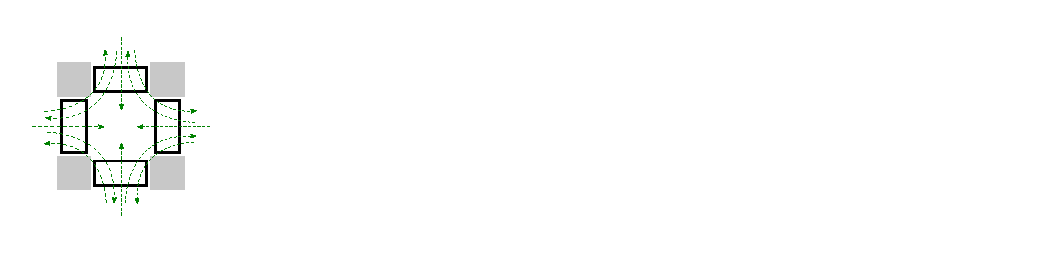
\includegraphics[width=\unitlength,page=1]{flow_path_model.pdf}}%
    \put(0.07466184,0.20939855){\color[rgb]{0,0,0}\makebox(0,0)[t]{\lineheight{0}\smash{\begin{tabular}[t]{c} $v^m_{i+1,j}$\end{tabular}}}}%
    \put(0.16223907,0.03849428){\color[rgb]{0,0,0}\makebox(0,0)[t]{\lineheight{0}\smash{\begin{tabular}[t]{c} $v^m_{i-1,j}$\end{tabular}}}}%
    \put(0.02732203,0.08519193){\color[rgb]{0,0,0}\makebox(0,0)[t]{\lineheight{0}\smash{\begin{tabular}[t]{c} $v^m_{i,j-1}$\end{tabular}}}}%
    \put(0.20888119,0.16425542){\color[rgb]{0,0,0}\makebox(0,0)[t]{\lineheight{0}\smash{\begin{tabular}[t]{c} $v^m_{i,j+1}$\end{tabular}}}}%
    \put(0.1167175,0.12421848){\color[rgb]{0,0,0}\makebox(0,0)[t]{\lineheight{0}\smash{\begin{tabular}[t]{c} $c^m_{i,j}$\end{tabular}}}}%
    \put(0.74426438,0.19486467){\color[rgb]{0,0,0}\makebox(0,0)[lt]{\begin{minipage}{0.2250259\unitlength}\centering  \end{minipage}}}%
    \put(0.11411867,0.00324755){\color[rgb]{0,0,0}\makebox(0,0)[t]{\lineheight{0}\smash{\begin{tabular}[t]{c}(a)\end{tabular}}}}%
    \put(0.23479095,0.03573213){\color[rgb]{0,0,0}\makebox(0,0)[t]{\lineheight{0}\smash{\begin{tabular}[t]{c} $v^1_{2,1}=1$\end{tabular}}}}%
    \put(0.23112447,0.01464194){\color[rgb]{0,0,0}\makebox(0,0)[t]{\lineheight{0}\smash{\begin{tabular}[t]{c} $c^1_{2,2}=1$\end{tabular}}}}%
    \put(0,0){\includegraphics[width=\unitlength,page=2]{flow_path_model.pdf}}%
    \put(0.47988729,0.18757502){\color[rgb]{0,0,0}\makebox(0,0)[t]{\lineheight{0}\smash{\begin{tabular}[t]{c}pressure\end{tabular}}}}%
    \put(0.47939149,0.17425488){\color[rgb]{0,0,0}\makebox(0,0)[t]{\lineheight{0}\smash{\begin{tabular}[t]{c}sensor\end{tabular}}}}%
    \put(0.21109423,0.06618444){\color[rgb]{0,0,0}\makebox(0,0)[lt]{\lineheight{0}\smash{\begin{tabular}[t]{l}pressure\end{tabular}}}}%
    \put(0.21332506,0.05256601){\color[rgb]{0,0,0}\makebox(0,0)[lt]{\lineheight{0}\smash{\begin{tabular}[t]{l}source\end{tabular}}}}%
    \put(0,0){\includegraphics[width=\unitlength,page=3]{flow_path_model.pdf}}%
    \put(0.35665285,0.0031953){\color[rgb]{0,0,0}\makebox(0,0)[t]{\lineheight{0}\smash{\begin{tabular}[t]{c}(b)\end{tabular}}}}%
    \put(0,0){\includegraphics[width=\unitlength,page=4]{flow_path_model.pdf}}%
    \put(0.29415113,0.00489445){\color[rgb]{0,0,0}\makebox(0,0)[t]{\lineheight{0}\smash{\begin{tabular}[t]{c} $v^1_{2,3}=1$\end{tabular}}}}%
    \put(0,0){\includegraphics[width=\unitlength,page=5]{flow_path_model.pdf}}%
    \put(0.4093913,0.02047866){\color[rgb]{0,0,0}\makebox(0,0)[t]{\lineheight{0}\smash{\begin{tabular}[t]{c} $v^1_{3,4}=1$\end{tabular}}}}%
    \put(0,0){\includegraphics[width=\unitlength,page=6]{flow_path_model.pdf}}%
    \put(0.34344779,0.02047866){\color[rgb]{0,0,0}\makebox(0,0)[t]{\lineheight{0}\smash{\begin{tabular}[t]{c} $c^1_{2,4}=1$\end{tabular}}}}%
    \put(0,0){\includegraphics[width=\unitlength,page=7]{flow_path_model.pdf}}%
    \put(0.46320451,0.22303412){\color[rgb]{0,0,0}\makebox(0,0)[t]{\lineheight{0}\smash{\begin{tabular}[t]{c} $v^1_{8,9}=1$\end{tabular}}}}%
    \put(0.38140477,0.22303412){\color[rgb]{0,0,0}\makebox(0,0)[t]{\lineheight{0}\smash{\begin{tabular}[t]{c} $v^1_{8,7}=1$\end{tabular}}}}%
    \put(0.47627753,0.13412483){\color[rgb]{0,0,0}\makebox(0,0)[t]{\lineheight{0}\smash{\begin{tabular}[t]{c} $v^1_{7,8}=0$\end{tabular}}}}%
    \put(0.42531984,0.24078875){\color[rgb]{0,0,0}\makebox(0,0)[t]{\lineheight{0}\smash{\begin{tabular}[t]{c} $c^1_{8,8}=1$\end{tabular}}}}%
    \put(0,0){\includegraphics[width=\unitlength,page=8]{flow_path_model.pdf}}%
    \put(0.23841261,0.09652239){\color[rgb]{0,0,0}\makebox(0,0)[t]{\lineheight{0}\smash{\begin{tabular}[t]{c} $v^1_{3,2}=0$\end{tabular}}}}%
    \put(0,0){\includegraphics[width=\unitlength,page=9]{flow_path_model.pdf}}%
    \put(0.60849977,0.00324755){\color[rgb]{0,0,0}\makebox(0,0)[t]{\lineheight{0}\smash{\begin{tabular}[t]{c}(c)\end{tabular}}}}%
    \put(0,0){\includegraphics[width=\unitlength,page=10]{flow_path_model.pdf}}%
    \put(0.84356671,0.0031953){\color[rgb]{0,0,0}\makebox(0,0)[t]{\lineheight{0}\smash{\begin{tabular}[t]{c}(d)\end{tabular}}}}%
    \put(0,0){\includegraphics[width=\unitlength,page=11]{flow_path_model.pdf}}%
    \put(0.81301938,0.16396088){\color[rgb]{0,0,0}\makebox(0,0)[t]{\lineheight{0}\smash{\begin{tabular}[t]{c}$i_1,j_1$\end{tabular}}}}%
    \put(0.83954185,0.20655999){\color[rgb]{0,0,0}\makebox(0,0)[t]{\lineheight{0}\smash{\begin{tabular}[t]{c}  $-f^m_{i_1,j_1+1}=f^m_{i_2,j_2-1}$\end{tabular}}}}%
    \put(0,0){\includegraphics[width=\unitlength,page=12]{flow_path_model.pdf}}%
    \put(0.85687381,0.04696493){\color[rgb]{0,0,0}\makebox(0,0)[t]{\lineheight{0}\smash{\begin{tabular}[t]{c}  $f^m_{i_4,j_4+1}=-f^m_{i_3,j_3-1}$\end{tabular}}}}%
    \put(0,0){\includegraphics[width=\unitlength,page=13]{flow_path_model.pdf}}%
    \put(0.94687866,0.10890966){\color[rgb]{0,0,0}\makebox(0,0)[t]{\lineheight{0}\smash{\begin{tabular}[t]{c}  $f^m_{i_3+1,j_3}$\end{tabular}}}}%
    \put(0.94973528,0.14275114){\color[rgb]{0,0,0}\makebox(0,0)[t]{\lineheight{0}\smash{\begin{tabular}[t]{c}$-f^m_{i_2-1,j_2}$\end{tabular}}}}%
    \put(0.94297016,0.12706598){\color[rgb]{0,0,0}\rotatebox{-90}{\makebox(0,0)[t]{\lineheight{0}\smash{\begin{tabular}[t]{c}=\end{tabular}}}}}%
    \put(0,0){\includegraphics[width=\unitlength,page=14]{flow_path_model.pdf}}%
    \put(0.73804713,0.10949702){\color[rgb]{0,0,0}\makebox(0,0)[t]{\lineheight{0}\smash{\begin{tabular}[t]{c} $-f^m_{i_4+1,j_4}$\end{tabular}}}}%
    \put(0.74720408,0.14518711){\color[rgb]{0,0,0}\makebox(0,0)[t]{\lineheight{0}\smash{\begin{tabular}[t]{c}$f^m_{i_1-1,j_1}$\end{tabular}}}}%
    \put(0.73712675,0.12950195){\color[rgb]{0,0,0}\rotatebox{-90}{\makebox(0,0)[t]{\lineheight{0}\smash{\begin{tabular}[t]{c}=\end{tabular}}}}}%
    \put(0.87714474,0.16396088){\color[rgb]{0,0,0}\makebox(0,0)[t]{\lineheight{0}\smash{\begin{tabular}[t]{c}$i_2,j_2$\end{tabular}}}}%
    \put(0.87714474,0.08750469){\color[rgb]{0,0,0}\makebox(0,0)[t]{\lineheight{0}\smash{\begin{tabular}[t]{c}$i_3,j_3$\end{tabular}}}}%
    \put(0.81301938,0.08750469){\color[rgb]{0,0,0}\makebox(0,0)[t]{\lineheight{0}\smash{\begin{tabular}[t]{c}$i_4,j_4$\end{tabular}}}}%
    \put(0,0){\includegraphics[width=\unitlength,page=15]{flow_path_model.pdf}}%
  \end{picture}%
\endgroup%
\label{fig:flow_path_model}
}
\end{figure*}
	\clearpage
\begin{figure*}[p]
{
\figurefontsize
  \begin{minipage}[b]{0.70\textwidth}
\centering
\begingroup%
  \makeatletter%
  \providecommand\color[2][]{%
    \errmessage{(Inkscape) Color is used for the text in Inkscape, but the package 'color.sty' is not loaded}%
    \renewcommand\color[2][]{}%
  }%
  \providecommand\transparent[1]{%
    \errmessage{(Inkscape) Transparency is used (non-zero) for the text in Inkscape, but the package 'transparent.sty' is not loaded}%
    \renewcommand\transparent[1]{}%
  }%
  \providecommand\rotatebox[2]{#2}%
  \newcommand*\fsize{\dimexpr\f@size pt\relax}%
  \newcommand*\lineheight[1]{\fontsize{\fsize}{#1\fsize}\selectfont}%
  \ifx\svgwidth\undefined%
    \setlength{\unitlength}{350.73833758bp}%
    \ifx\svgscale\undefined%
      \relax%
    \else%
      \setlength{\unitlength}{\unitlength * \real{\svgscale}}%
    \fi%
  \else%
    \setlength{\unitlength}{\svgwidth}%
  \fi%
  \global\let\svgwidth\undefined%
  \global\let\svgscale\undefined%
  \makeatother%
  \begin{picture}(1,0.34585323)%
    \lineheight{1}%
    \setlength\tabcolsep{0pt}%
    \put(0,0){\includegraphics[width=\unitlength,page=1]{minimum_loops.pdf}}%
    \put(0.13336499,0.00457322){\color[rgb]{0,0,0}\makebox(0,0)[t]{\lineheight{0}\smash{\begin{tabular}[t]{c}(a)\end{tabular}}}}%
    \put(0,0){\includegraphics[width=\unitlength,page=2]{minimum_loops.pdf}}%
    \put(0.12333027,0.33079514){\color[rgb]{0,0,0}\makebox(0,0)[t]{\lineheight{0}\smash{\begin{tabular}[t]{c}test path with a loop\end{tabular}}}}%
    \put(0,0){\includegraphics[width=\unitlength,page=3]{minimum_loops.pdf}}%
    \put(0.4987876,0.00485983){\color[rgb]{0,0,0}\makebox(0,0)[t]{\lineheight{0}\smash{\begin{tabular}[t]{c}(b)\end{tabular}}}}%
    \put(0,0){\includegraphics[width=\unitlength,page=4]{minimum_loops.pdf}}%
    \put(0.40323992,0.02760691){\color[rgb]{0,0,0}\makebox(0,0)[t]{\lineheight{0}\smash{\begin{tabular}[t]{c}uncovered valves\end{tabular}}}}%
    \put(0,0){\includegraphics[width=\unitlength,page=5]{minimum_loops.pdf}}%
    \put(0.49953924,0.3309203){\color[rgb]{0,0,0}\makebox(0,0)[t]{\lineheight{0}\smash{\begin{tabular}[t]{c}altered  test path\end{tabular}}}}%
    \put(0,0){\includegraphics[width=\unitlength,page=6]{minimum_loops.pdf}}%
    \put(0.8626287,0.00485983){\color[rgb]{0,0,0}\makebox(0,0)[t]{\lineheight{0}\smash{\begin{tabular}[t]{c}(c)\end{tabular}}}}%
    \put(0,0){\includegraphics[width=\unitlength,page=7]{minimum_loops.pdf}}%
    \put(0.86244389,0.33100592){\color[rgb]{0,0,0}\makebox(0,0)[t]{\lineheight{0}\smash{\begin{tabular}[t]{c}additional test path\end{tabular}}}}%
    \put(0,0){\includegraphics[width=\unitlength,page=8]{minimum_loops.pdf}}%
  \end{picture}%
\endgroup%
\label{fig:minimum_loops}
\end{minipage}
\hspace{10pt}
  \begin{minipage}[b]{0.28\textwidth}
\hskip 30pt%
\begingroup%
  \makeatletter%
  \providecommand\color[2][]{%
    \errmessage{(Inkscape) Color is used for the text in Inkscape, but the package 'color.sty' is not loaded}%
    \renewcommand\color[2][]{}%
  }%
  \providecommand\transparent[1]{%
    \errmessage{(Inkscape) Transparency is used (non-zero) for the text in Inkscape, but the package 'transparent.sty' is not loaded}%
    \renewcommand\transparent[1]{}%
  }%
  \providecommand\rotatebox[2]{#2}%
  \newcommand*\fsize{\dimexpr\f@size pt\relax}%
  \newcommand*\lineheight[1]{\fontsize{\fsize}{#1\fsize}\selectfont}%
  \ifx\svgwidth\undefined%
    \setlength{\unitlength}{386.82426453bp}%
    \ifx\svgscale\undefined%
      \relax%
    \else%
      \setlength{\unitlength}{\unitlength * \real{\svgscale}}%
    \fi%
  \else%
    \setlength{\unitlength}{\svgwidth}%
  \fi%
  \global\let\svgwidth\undefined%
  \global\let\svgscale\undefined%
  \makeatother%
  \begin{picture}(1,0.26753172)%
    \lineheight{1}%
    \setlength\tabcolsep{0pt}%
    \put(0,0){\includegraphics[width=\unitlength,page=1]{cut_var.pdf}}%
    \put(0.03545624,0.13380183){\color[rgb]{0,0,0}\makebox(0,0)[t]{\lineheight{0}\smash{\begin{tabular}[t]{c} $v^m_{i,j-1}$\end{tabular}}}}%
    \put(0.09432523,0.19059469){\color[rgb]{0,0,0}\makebox(0,0)[t]{\lineheight{0}\smash{\begin{tabular}[t]{c} $v^m_{i+1,j}$\end{tabular}}}}%
    \put(0.85398918,0.28325158){\color[rgb]{0,0,0}\makebox(0,0)[lt]{\begin{minipage}{0.29201976\unitlength}\centering  \end{minipage}}}%
    \put(0,0){\includegraphics[width=\unitlength,page=2]{cut_var.pdf}}%
    \put(0.15156589,0.13372077){\color[rgb]{0,0,0}\makebox(0,0)[t]{\lineheight{0}\smash{\begin{tabular}[t]{c} $v^m_{i,j+1}$\end{tabular}}}}%
    \put(0,0){\includegraphics[width=\unitlength,page=3]{cut_var.pdf}}%
    \put(0.09432523,0.13372077){\color[rgb]{0,0,0}\makebox(0,0)[t]{\lineheight{0}\smash{\begin{tabular}[t]{c} $c_{i,j}$\end{tabular}}}}%
    \put(0,0){\includegraphics[width=\unitlength,page=4]{cut_var.pdf}}%
    \put(0.09432523,0.07576842){\color[rgb]{0,0,0}\makebox(0,0)[t]{\lineheight{0}\smash{\begin{tabular}[t]{c} $v^m_{i-1,j}$\end{tabular}}}}%
    \put(0,0){\includegraphics[width=\unitlength,page=5]{cut_var.pdf}}%
    \put(0.09432523,0.0176433){\color[rgb]{0,0,0}\makebox(0,0)[t]{\lineheight{0}\smash{\begin{tabular}[t]{c} $c_{i-2,j}$\end{tabular}}}}%
    \put(0.1892453,0.0607137){\color[rgb]{0,0,0}\makebox(0,0)[t]{\lineheight{0}\smash{\begin{tabular}[t]{c}obstacle \end{tabular}}}}%
    \put(0.2898603,-0.1008234){\color[rgb]{0,0,0}\makebox(0,0)[lt]{\begin{minipage}{0.24914414\unitlength}\raggedright \end{minipage}}}%
    \put(0,0){\includegraphics[width=\unitlength,page=6]{cut_var.pdf}}%
    \put(0.18965712,0.04042579){\color[rgb]{0,0,0}\makebox(0,0)[t]{\lineheight{1.25}\smash{\begin{tabular}[t]{c}blocks\end{tabular}}}}%
  \end{picture}%
\endgroup%
\vspace{10pt}
    \label{fig:cut_var}
  \end{minipage}
}
\end{figure*}
	\clearpage
\begin{figure}[p]
{\figurefontsize
  \begin{minipage}[b]{0.20\textwidth}
    \centering
\begingroup%
  \makeatletter%
  \providecommand\color[2][]{%
    \errmessage{(Inkscape) Color is used for the text in Inkscape, but the package 'color.sty' is not loaded}%
    \renewcommand\color[2][]{}%
  }%
  \providecommand\transparent[1]{%
    \errmessage{(Inkscape) Transparency is used (non-zero) for the text in Inkscape, but the package 'transparent.sty' is not loaded}%
    \renewcommand\transparent[1]{}%
  }%
  \providecommand\rotatebox[2]{#2}%
  \newcommand*\fsize{\dimexpr\f@size pt\relax}%
  \newcommand*\lineheight[1]{\fontsize{\fsize}{#1\fsize}\selectfont}%
  \ifx\svgwidth\undefined%
    \setlength{\unitlength}{276.32522063bp}%
    \ifx\svgscale\undefined%
      \relax%
    \else%
      \setlength{\unitlength}{\unitlength * \real{\svgscale}}%
    \fi%
  \else%
    \setlength{\unitlength}{\svgwidth}%
  \fi%
  \global\let\svgwidth\undefined%
  \global\let\svgscale\undefined%
  \makeatother%
  \begin{picture}(1,0.41580668)%
    \lineheight{1}%
    \setlength\tabcolsep{0pt}%
    \put(0.79560125,0.43781273){\color[rgb]{0,0,0}\makebox(0,0)[lt]{\begin{minipage}{0.40879485\unitlength}\centering  \end{minipage}}}%
    \put(0,0){\includegraphics[width=\unitlength,page=1]{control_test.pdf}}%
    \put(0.21758564,0.39470404){\color[rgb]{0,0,0}\makebox(0,0)[t]{\lineheight{0}\smash{\begin{tabular}[t]{c}control leakage not tested\end{tabular}}}}%
    \put(0.17969279,0.00585778){\color[rgb]{0,0,0}\makebox(0,0)[t]{\lineheight{0}\smash{\begin{tabular}[t]{c}control leakage tested \end{tabular}}}}%
  \end{picture}%
\endgroup%
    \label{fig:control_test}
  \end{minipage}
  \hspace{14pt}
  \begin{minipage}[b]{0.25\textwidth}
\centering
\begingroup%
  \makeatletter%
  \providecommand\color[2][]{%
    \errmessage{(Inkscape) Color is used for the text in Inkscape, but the package 'color.sty' is not loaded}%
    \renewcommand\color[2][]{}%
  }%
  \providecommand\transparent[1]{%
    \errmessage{(Inkscape) Transparency is used (non-zero) for the text in Inkscape, but the package 'transparent.sty' is not loaded}%
    \renewcommand\transparent[1]{}%
  }%
  \providecommand\rotatebox[2]{#2}%
  \newcommand*\fsize{\dimexpr\f@size pt\relax}%
  \newcommand*\lineheight[1]{\fontsize{\fsize}{#1\fsize}\selectfont}%
  \ifx\svgwidth\undefined%
    \setlength{\unitlength}{128.98988861bp}%
    \ifx\svgscale\undefined%
      \relax%
    \else%
      \setlength{\unitlength}{\unitlength * \real{\svgscale}}%
    \fi%
  \else%
    \setlength{\unitlength}{\svgwidth}%
  \fi%
  \global\let\svgwidth\undefined%
  \global\let\svgscale\undefined%
  \makeatother%
  \begin{picture}(1,0.88003908)%
    \lineheight{1}%
    \setlength\tabcolsep{0pt}%
    \put(0,0){\includegraphics[width=\unitlength,page=1]{long_channel.pdf}}%
    \put(0.01307636,0.83966754){\color[rgb]{0,0,0}\makebox(0,0)[lt]{\lineheight{0}\smash{\begin{tabular}[t]{l}leakage at the missing valve\end{tabular}}}}%
    \put(0,0){\includegraphics[width=\unitlength,page=2]{long_channel.pdf}}%
    \put(0.89413656,0.42781522){\color[rgb]{0,0,0}\makebox(0,0)[t]{\lineheight{0}\smash{\begin{tabular}[t]{c}missing\end{tabular}}}}%
    \put(0.89220706,0.3759774){\color[rgb]{0,0,0}\makebox(0,0)[t]{\lineheight{0}\smash{\begin{tabular}[t]{c}vavle\end{tabular}}}}%
    \put(0.89606602,0.68238546){\color[rgb]{0,0,0}\makebox(0,0)[t]{\lineheight{0}\smash{\begin{tabular}[t]{c}test\end{tabular}}}}%
    \put(0.89413652,0.63054765){\color[rgb]{0,0,0}\makebox(0,0)[t]{\lineheight{0}\smash{\begin{tabular}[t]{c}path\end{tabular}}}}%
    \put(0,0){\includegraphics[width=\unitlength,page=3]{long_channel.pdf}}%
    \put(0.8953705,0.1556354){\color[rgb]{0,0,0}\makebox(0,0)[t]{\lineheight{0}\smash{\begin{tabular}[t]{c}long\end{tabular}}}}%
    \put(0.893441,0.10379758){\color[rgb]{0,0,0}\makebox(0,0)[t]{\lineheight{0}\smash{\begin{tabular}[t]{c}channel\end{tabular}}}}%
    \put(0,0){\includegraphics[width=\unitlength,page=4]{long_channel.pdf}}%
    \put(0.26019297,0.00079494){\color[rgb]{0,0,0}\makebox(0,0)[t]{\lineheight{0}\smash{\begin{tabular}[t]{c}valves not tested\end{tabular}}}}%
  \end{picture}%
\endgroup%
\label{fig:long_channel}
  \end{minipage}
}
\end{figure}
	\clearpage
\begin{figure}[p]
{\figurefontsize
\centering
\begingroup%
  \makeatletter%
  \providecommand\color[2][]{%
    \errmessage{(Inkscape) Color is used for the text in Inkscape, but the package 'color.sty' is not loaded}%
    \renewcommand\color[2][]{}%
  }%
  \providecommand\transparent[1]{%
    \errmessage{(Inkscape) Transparency is used (non-zero) for the text in Inkscape, but the package 'transparent.sty' is not loaded}%
    \renewcommand\transparent[1]{}%
  }%
  \providecommand\rotatebox[2]{#2}%
  \newcommand*\fsize{\dimexpr\f@size pt\relax}%
  \newcommand*\lineheight[1]{\fontsize{\fsize}{#1\fsize}\selectfont}%
  \ifx\svgwidth\undefined%
    \setlength{\unitlength}{211.82343716bp}%
    \ifx\svgscale\undefined%
      \relax%
    \else%
      \setlength{\unitlength}{\unitlength * \real{\svgscale}}%
    \fi%
  \else%
    \setlength{\unitlength}{\svgwidth}%
  \fi%
  \global\let\svgwidth\undefined%
  \global\let\svgscale\undefined%
  \makeatother%
  \begin{picture}(1,1.07614404)%
    \lineheight{1}%
    \setlength\tabcolsep{0pt}%
    \put(0,0){\includegraphics[width=\unitlength,page=1]{supper_cell.pdf}}%
    \put(0.57284384,0.56105416){\color[rgb]{0,0,0}\makebox(0,0)[lt]{\lineheight{0}\smash{\begin{tabular}[t]{l}collapse\end{tabular}}}}%
    \put(0,0){\includegraphics[width=\unitlength,page=2]{supper_cell.pdf}}%
    \put(0.5923176,1.0515598){\color[rgb]{0,0,0}\makebox(0,0)[lt]{\lineheight{0}\smash{\begin{tabular}[t]{l}missing valve\end{tabular}}}}%
    \put(0,0){\includegraphics[width=\unitlength,page=3]{supper_cell.pdf}}%
    \put(0.02850614,1.0515598){\color[rgb]{0,0,0}\makebox(0,0)[lt]{\lineheight{0}\smash{\begin{tabular}[t]{l}missing valve\end{tabular}}}}%
    \put(0,0){\includegraphics[width=\unitlength,page=4]{supper_cell.pdf}}%
    \put(0.20637887,0.55586999){\color[rgb]{0,0,0}\makebox(0,0)[t]{\lineheight{0}\smash{\begin{tabular}[t]{c}(a)\end{tabular}}}}%
    \put(0.77519232,0.55586999){\color[rgb]{0,0,0}\makebox(0,0)[t]{\lineheight{0}\smash{\begin{tabular}[t]{c}(b)\end{tabular}}}}%
    \put(0,0){\includegraphics[width=\unitlength,page=5]{supper_cell.pdf}}%
    \put(0.20724264,0.00757236){\color[rgb]{0,0,0}\makebox(0,0)[t]{\lineheight{0}\smash{\begin{tabular}[t]{c}(c)\end{tabular}}}}%
    \put(0.76543405,0.00757236){\color[rgb]{0,0,0}\makebox(0,0)[t]{\lineheight{0}\smash{\begin{tabular}[t]{c}(d)\end{tabular}}}}%
    \put(0,0){\includegraphics[width=\unitlength,page=6]{supper_cell.pdf}}%
    \put(0.03567827,0.50322759){\color[rgb]{0,0,0}\makebox(0,0)[lt]{\lineheight{0}\smash{\begin{tabular}[t]{l}super cell\end{tabular}}}}%
  \end{picture}%
\endgroup%
\label{fig:super_cell}
}
\end{figure}
	\clearpage
\begin{figure}[p]
{ \figurefontsize
\centering
\begingroup%
  \makeatletter%
  \providecommand\color[2][]{%
    \errmessage{(Inkscape) Color is used for the text in Inkscape, but the package 'color.sty' is not loaded}%
    \renewcommand\color[2][]{}%
  }%
  \providecommand\transparent[1]{%
    \errmessage{(Inkscape) Transparency is used (non-zero) for the text in Inkscape, but the package 'transparent.sty' is not loaded}%
    \renewcommand\transparent[1]{}%
  }%
  \providecommand\rotatebox[2]{#2}%
  \newcommand*\fsize{\dimexpr\f@size pt\relax}%
  \newcommand*\lineheight[1]{\fontsize{\fsize}{#1\fsize}\selectfont}%
  \ifx\svgwidth\undefined%
    \setlength{\unitlength}{251.91578887bp}%
    \ifx\svgscale\undefined%
      \relax%
    \else%
      \setlength{\unitlength}{\unitlength * \real{\svgscale}}%
    \fi%
  \else%
    \setlength{\unitlength}{\svgwidth}%
  \fi%
  \global\let\svgwidth\undefined%
  \global\let\svgscale\undefined%
  \makeatother%
  \begin{picture}(1,0.48923111)%
    \lineheight{1}%
    \setlength\tabcolsep{0pt}%
    \put(0,0){\includegraphics[width=\unitlength,page=1]{multi_port_test_example.pdf}}%
    \put(0.5422674,0.37811017){\color[rgb]{0,0,0}\makebox(0,0)[t]{\lineheight{0}\smash{\begin{tabular}[t]{c}pressure\end{tabular}}}}%
    \put(0.54127943,0.35156736){\color[rgb]{0,0,0}\makebox(0,0)[t]{\lineheight{0}\smash{\begin{tabular}[t]{c}sensor1\end{tabular}}}}%
    \put(0.00010176,0.13348635){\color[rgb]{0,0,0}\makebox(0,0)[lt]{\lineheight{0}\smash{\begin{tabular}[t]{l}pressure\end{tabular}}}}%
    \put(0.00454709,0.10634897){\color[rgb]{0,0,0}\makebox(0,0)[lt]{\lineheight{0}\smash{\begin{tabular}[t]{l}source\end{tabular}}}}%
    \put(0,0){\includegraphics[width=\unitlength,page=2]{multi_port_test_example.pdf}}%
    \put(0.20833629,0.46855944){\color[rgb]{0,0,0}\makebox(0,0)[t]{\lineheight{0}\smash{\begin{tabular}[t]{c}valves under test\end{tabular}}}}%
    \put(0,0){\includegraphics[width=\unitlength,page=3]{multi_port_test_example.pdf}}%
    \put(0.29285126,0.00657565){\color[rgb]{0,0,0}\makebox(0,0)[t]{\lineheight{0}\smash{\begin{tabular}[t]{c}(a)\end{tabular}}}}%
    \put(0.82201525,0.00636722){\color[rgb]{0,0,0}\makebox(0,0)[t]{\lineheight{0}\smash{\begin{tabular}[t]{c}(b)\end{tabular}}}}%
    \put(0,0){\includegraphics[width=\unitlength,page=4]{multi_port_test_example.pdf}}%
    \put(0.54235783,0.13122353){\color[rgb]{0,0,0}\makebox(0,0)[t]{\lineheight{0}\smash{\begin{tabular}[t]{c}pressure\end{tabular}}}}%
    \put(0.54136985,0.10468071){\color[rgb]{0,0,0}\makebox(0,0)[t]{\lineheight{0}\smash{\begin{tabular}[t]{c}sensor2\end{tabular}}}}%
    \put(0,0){\includegraphics[width=\unitlength,page=5]{multi_port_test_example.pdf}}%
    \put(0.79633358,0.46855944){\color[rgb]{0,0,0}\makebox(0,0)[t]{\lineheight{0}\smash{\begin{tabular}[t]{c}valve under test\end{tabular}}}}%
    \put(0,0){\includegraphics[width=\unitlength,page=6]{multi_port_test_example.pdf}}%
    \put(0.12641208,0.02182173){\color[rgb]{0,0,0}\makebox(0,0)[t]{\lineheight{0}\smash{\begin{tabular}[t]{c}branching point\end{tabular}}}}%
    \put(0,0){\includegraphics[width=\unitlength,page=7]{multi_port_test_example.pdf}}%
  \end{picture}%
\endgroup%
\label{fig:multi_port_test_example}
}
\end{figure}
	\clearpage
\begin{figure}[p]
{\figurefontsize
\centering
\begingroup%
  \makeatletter%
  \providecommand\color[2][]{%
    \errmessage{(Inkscape) Color is used for the text in Inkscape, but the package 'color.sty' is not loaded}%
    \renewcommand\color[2][]{}%
  }%
  \providecommand\transparent[1]{%
    \errmessage{(Inkscape) Transparency is used (non-zero) for the text in Inkscape, but the package 'transparent.sty' is not loaded}%
    \renewcommand\transparent[1]{}%
  }%
  \providecommand\rotatebox[2]{#2}%
  \newcommand*\fsize{\dimexpr\f@size pt\relax}%
  \newcommand*\lineheight[1]{\fontsize{\fsize}{#1\fsize}\selectfont}%
  \ifx\svgwidth\undefined%
    \setlength{\unitlength}{149.68376459bp}%
    \ifx\svgscale\undefined%
      \relax%
    \else%
      \setlength{\unitlength}{\unitlength * \real{\svgscale}}%
    \fi%
  \else%
    \setlength{\unitlength}{\svgwidth}%
  \fi%
  \global\let\svgwidth\undefined%
  \global\let\svgscale\undefined%
  \makeatother%
  \begin{picture}(1,0.66600079)%
    \lineheight{1}%
    \setlength\tabcolsep{0pt}%
    \put(0,0){\includegraphics[width=\unitlength,page=1]{joint_loops.pdf}}%
    \put(0.91776559,0.50781178){\color[rgb]{0,0,0}\makebox(0,0)[t]{\lineheight{0}\smash{\begin{tabular}[t]{c}pressure\end{tabular}}}}%
    \put(0.91610285,0.46314058){\color[rgb]{0,0,0}\makebox(0,0)[t]{\lineheight{0}\smash{\begin{tabular}[t]{c}sensor1\end{tabular}}}}%
    \put(0.00017126,0.10065394){\color[rgb]{0,0,0}\makebox(0,0)[lt]{\lineheight{0}\smash{\begin{tabular}[t]{l}pressure\end{tabular}}}}%
    \put(0.0076527,0.05498209){\color[rgb]{0,0,0}\makebox(0,0)[lt]{\lineheight{0}\smash{\begin{tabular}[t]{l}source\end{tabular}}}}%
    \put(0,0){\includegraphics[width=\unitlength,page=2]{joint_loops.pdf}}%
    \put(0.91791777,0.10263139){\color[rgb]{0,0,0}\makebox(0,0)[t]{\lineheight{0}\smash{\begin{tabular}[t]{c}pressure\end{tabular}}}}%
    \put(0.91625503,0.05796019){\color[rgb]{0,0,0}\makebox(0,0)[t]{\lineheight{0}\smash{\begin{tabular}[t]{c}sensor3\end{tabular}}}}%
    \put(0,0){\includegraphics[width=\unitlength,page=3]{joint_loops.pdf}}%
    \put(0.91791777,0.37174367){\color[rgb]{0,0,0}\makebox(0,0)[t]{\lineheight{0}\smash{\begin{tabular}[t]{c}pressure\end{tabular}}}}%
    \put(0.91625503,0.32707246){\color[rgb]{0,0,0}\makebox(0,0)[t]{\lineheight{0}\smash{\begin{tabular}[t]{c}sensor2\end{tabular}}}}%
    \put(0,0){\includegraphics[width=\unitlength,page=4]{joint_loops.pdf}}%
    \put(0.30523075,0.63121065){\color[rgb]{0,0,0}\makebox(0,0)[lt]{\lineheight{0}\smash{\begin{tabular}[t]{l}loop\end{tabular}}}}%
    \put(0,0){\includegraphics[width=\unitlength,page=5]{joint_loops.pdf}}%
    \put(0.5062478,0.63121065){\color[rgb]{0,0,0}\makebox(0,0)[lt]{\lineheight{0}\smash{\begin{tabular}[t]{l}fault masked\end{tabular}}}}%
    \put(0,0){\includegraphics[width=\unitlength,page=6]{joint_loops.pdf}}%
  \end{picture}%
\endgroup%
\label{fig:joint_loops}
}
\end{figure}
	\clearpage
\begin{figure}[p]
{\figurefontsize
\centering
\begingroup%
  \makeatletter%
  \providecommand\color[2][]{%
    \errmessage{(Inkscape) Color is used for the text in Inkscape, but the package 'color.sty' is not loaded}%
    \renewcommand\color[2][]{}%
  }%
  \providecommand\transparent[1]{%
    \errmessage{(Inkscape) Transparency is used (non-zero) for the text in Inkscape, but the package 'transparent.sty' is not loaded}%
    \renewcommand\transparent[1]{}%
  }%
  \providecommand\rotatebox[2]{#2}%
  \newcommand*\fsize{\dimexpr\f@size pt\relax}%
  \newcommand*\lineheight[1]{\fontsize{\fsize}{#1\fsize}\selectfont}%
  \ifx\svgwidth\undefined%
    \setlength{\unitlength}{164.36218977bp}%
    \ifx\svgscale\undefined%
      \relax%
    \else%
      \setlength{\unitlength}{\unitlength * \real{\svgscale}}%
    \fi%
  \else%
    \setlength{\unitlength}{\svgwidth}%
  \fi%
  \global\let\svgwidth\undefined%
  \global\let\svgscale\undefined%
  \makeatother%
  \begin{picture}(1,0.66862782)%
    \lineheight{1}%
    \setlength\tabcolsep{0pt}%
    \put(0,0){\includegraphics[width=\unitlength,page=1]{multi_port_cut_theorem.pdf}}%
    \put(0.11106126,0.0928715){\color[rgb]{0,0,0}\makebox(0,0)[lt]{\lineheight{0}\smash{\begin{tabular}[t]{l}pressure\end{tabular}}}}%
    \put(0.11787443,0.0512784){\color[rgb]{0,0,0}\makebox(0,0)[lt]{\lineheight{0}\smash{\begin{tabular}[t]{l}source\end{tabular}}}}%
    \put(0,0){\includegraphics[width=\unitlength,page=2]{multi_port_cut_theorem.pdf}}%
    \put(0.92510957,0.46069704){\color[rgb]{0,0,0}\makebox(0,0)[t]{\lineheight{0}\smash{\begin{tabular}[t]{c}pressure\end{tabular}}}}%
    \put(0.92359532,0.42001521){\color[rgb]{0,0,0}\makebox(0,0)[t]{\lineheight{0}\smash{\begin{tabular}[t]{c}sensor1\end{tabular}}}}%
    \put(0,0){\includegraphics[width=\unitlength,page=3]{multi_port_cut_theorem.pdf}}%
    \put(0.92524815,0.0928715){\color[rgb]{0,0,0}\makebox(0,0)[t]{\lineheight{0}\smash{\begin{tabular}[t]{c}pressure\end{tabular}}}}%
    \put(0.9237339,0.05218968){\color[rgb]{0,0,0}\makebox(0,0)[t]{\lineheight{0}\smash{\begin{tabular}[t]{c}sensor2\end{tabular}}}}%
    \put(0.57966565,0.6337763){\color[rgb]{0,0,0}\makebox(0,0)[lt]{\lineheight{0}\smash{\begin{tabular}[t]{l}cell reachable \end{tabular}}}}%
    \put(0,0){\includegraphics[width=\unitlength,page=4]{multi_port_cut_theorem.pdf}}%
    \put(-0.00166363,0.45385357){\color[rgb]{0,0,0}\makebox(0,0)[lt]{\lineheight{0}\smash{\begin{tabular}[t]{l}cell reachable \end{tabular}}}}%
    \put(0,0){\includegraphics[width=\unitlength,page=5]{multi_port_cut_theorem.pdf}}%
    \put(0.58150381,0.59243274){\color[rgb]{0,0,0}\makebox(0,0)[lt]{\lineheight{1.25}\smash{\begin{tabular}[t]{l}from pressure sensor\end{tabular}}}}%
    \put(0.18721401,0.58891238){\color[rgb]{0,0,0}\makebox(0,0)[lt]{\lineheight{0}\smash{\begin{tabular}[t]{l}valve on the cut\end{tabular}}}}%
    \put(0,0){\includegraphics[width=\unitlength,page=6]{multi_port_cut_theorem.pdf}}%
    \put(0.00011883,0.41231393){\color[rgb]{0,0,0}\makebox(0,0)[lt]{\lineheight{1.25}\smash{\begin{tabular}[t]{l}from pressure \end{tabular}}}}%
    \put(-0.00237661,0.37023678){\color[rgb]{0,0,0}\makebox(0,0)[lt]{\lineheight{1.25}\smash{\begin{tabular}[t]{l}source\end{tabular}}}}%
  \end{picture}%
\endgroup%
\label{fig:multi_port_cut_theorem}
}
\end{figure}
	\clearpage
\begin{figure}[p]
{\figurefontsize
\centering
\begingroup%
  \makeatletter%
  \providecommand\color[2][]{%
    \errmessage{(Inkscape) Color is used for the text in Inkscape, but the package 'color.sty' is not loaded}%
    \renewcommand\color[2][]{}%
  }%
  \providecommand\transparent[1]{%
    \errmessage{(Inkscape) Transparency is used (non-zero) for the text in Inkscape, but the package 'transparent.sty' is not loaded}%
    \renewcommand\transparent[1]{}%
  }%
  \providecommand\rotatebox[2]{#2}%
  \newcommand*\fsize{\dimexpr\f@size pt\relax}%
  \newcommand*\lineheight[1]{\fontsize{\fsize}{#1\fsize}\selectfont}%
  \ifx\svgwidth\undefined%
    \setlength{\unitlength}{211.05656027bp}%
    \ifx\svgscale\undefined%
      \relax%
    \else%
      \setlength{\unitlength}{\unitlength * \real{\svgscale}}%
    \fi%
  \else%
    \setlength{\unitlength}{\svgwidth}%
  \fi%
  \global\let\svgwidth\undefined%
  \global\let\svgscale\undefined%
  \makeatother%
  \begin{picture}(1,0.65436127)%
    \lineheight{1}%
    \setlength\tabcolsep{0pt}%
    \put(0.75997541,0.02547154){\color[rgb]{0,0,0}\makebox(0,0)[lt]{\begin{minipage}{0.64296628\unitlength}\raggedright  \end{minipage}}}%
    \put(0.43135303,0.36053208){\color[rgb]{0,0,0}\makebox(0,0)[t]{\lineheight{0}\smash{\begin{tabular}[t]{c}(a)\end{tabular}}}}%
    \put(0.43135303,0.02036213){\color[rgb]{0,0,0}\makebox(0,0)[t]{\lineheight{0}\smash{\begin{tabular}[t]{c}(b)\end{tabular}}}}%
    \put(0,0){\includegraphics[width=\unitlength,page=1]{trees_cuts_traditional.pdf}}%
    \put(0.33859554,0.61002112){\color[rgb]{1,1,1}\makebox(0,0)[t]{\lineheight{0}\smash{\begin{tabular}[t]{c}c\end{tabular}}}}%
    \put(0,0){\includegraphics[width=\unitlength,page=2]{trees_cuts_traditional.pdf}}%
    \put(0.39502189,0.62528997){\color[rgb]{1,1,1}\makebox(0,0)[t]{\lineheight{0}\smash{\begin{tabular}[t]{c}d\end{tabular}}}}%
    \put(0,0){\includegraphics[width=\unitlength,page=3]{trees_cuts_traditional.pdf}}%
    \put(0.45144824,0.61002112){\color[rgb]{1,1,1}\makebox(0,0)[t]{\lineheight{0}\smash{\begin{tabular}[t]{c}e\end{tabular}}}}%
    \put(0,0){\includegraphics[width=\unitlength,page=4]{trees_cuts_traditional.pdf}}%
    \put(0.29398492,0.54820873){\color[rgb]{1,1,1}\makebox(0,0)[t]{\lineheight{0}\smash{\begin{tabular}[t]{c}b\end{tabular}}}}%
    \put(0,0){\includegraphics[width=\unitlength,page=5]{trees_cuts_traditional.pdf}}%
    \put(0.29398492,0.480717){\color[rgb]{1,1,1}\makebox(0,0)[t]{\lineheight{0}\smash{\begin{tabular}[t]{c}g\end{tabular}}}}%
    \put(0,0){\includegraphics[width=\unitlength,page=6]{trees_cuts_traditional.pdf}}%
    \put(0.50273409,0.54814853){\color[rgb]{1,1,1}\makebox(0,0)[t]{\lineheight{0}\smash{\begin{tabular}[t]{c}f\end{tabular}}}}%
    \put(0,0){\includegraphics[width=\unitlength,page=7]{trees_cuts_traditional.pdf}}%
    \put(0.50273409,0.47753461){\color[rgb]{1,1,1}\makebox(0,0)[t]{\lineheight{0}\smash{\begin{tabular}[t]{c}h\end{tabular}}}}%
    \put(0,0){\includegraphics[width=\unitlength,page=8]{trees_cuts_traditional.pdf}}%
    \put(0.21416078,0.51467423){\color[rgb]{1,1,1}\makebox(0,0)[t]{\lineheight{0}\smash{\begin{tabular}[t]{c}a\end{tabular}}}}%
    \put(0,0){\includegraphics[width=\unitlength,page=9]{trees_cuts_traditional.pdf}}%
    \put(0.58420569,0.51467423){\color[rgb]{1,1,1}\makebox(0,0)[t]{\lineheight{0}\smash{\begin{tabular}[t]{c}i\end{tabular}}}}%
    \put(0,0){\includegraphics[width=\unitlength,page=10]{trees_cuts_traditional.pdf}}%
    \put(0.6578201,0.55083915){\color[rgb]{1,1,1}\makebox(0,0)[t]{\lineheight{0}\smash{\begin{tabular}[t]{c}j\end{tabular}}}}%
    \put(0,0){\includegraphics[width=\unitlength,page=11]{trees_cuts_traditional.pdf}}%
    \put(0.6578201,0.47753461){\color[rgb]{1,1,1}\makebox(0,0)[t]{\lineheight{0}\smash{\begin{tabular}[t]{c}k\end{tabular}}}}%
    \put(0,0){\includegraphics[width=\unitlength,page=12]{trees_cuts_traditional.pdf}}%
    \put(0.04790939,0.61191036){\color[rgb]{0,0,0}\makebox(0,0)[lt]{\lineheight{0}\smash{\begin{tabular}[t]{l}pressure \end{tabular}}}}%
    \put(0.04911409,0.57507057){\color[rgb]{0,0,0}\makebox(0,0)[lt]{\lineheight{0}\smash{\begin{tabular}[t]{l}source\end{tabular}}}}%
    \put(0,0){\includegraphics[width=\unitlength,page=13]{trees_cuts_traditional.pdf}}%
    \put(0.77447189,0.58328518){\color[rgb]{1,1,1}\makebox(0,0)[t]{\lineheight{0}\smash{\begin{tabular}[t]{c}$O_1$\end{tabular}}}}%
    \put(0,0){\includegraphics[width=\unitlength,page=14]{trees_cuts_traditional.pdf}}%
    \put(0.77447189,0.44714196){\color[rgb]{1,1,1}\makebox(0,0)[t]{\lineheight{0}\smash{\begin{tabular}[t]{c}$O_2$\end{tabular}}}}%
    \put(0.3505303,0.51219196){\color[rgb]{0,0,0}\makebox(0,0)[lt]{\lineheight{0}\smash{\begin{tabular}[t]{l}mixer\end{tabular}}}}%
    \put(0.85704204,0.53094243){\color[rgb]{0,0,0}\makebox(0,0)[lt]{\lineheight{0}\smash{\begin{tabular}[t]{l}pressure \end{tabular}}}}%
    \put(0.85824681,0.49410267){\color[rgb]{0,0,0}\makebox(0,0)[lt]{\lineheight{0}\smash{\begin{tabular}[t]{l}sensors\end{tabular}}}}%
    \put(0,0){\includegraphics[width=\unitlength,page=15]{trees_cuts_traditional.pdf}}%
    \put(0.33859491,0.26867675){\color[rgb]{1,1,1}\makebox(0,0)[t]{\lineheight{0}\smash{\begin{tabular}[t]{c}c\end{tabular}}}}%
    \put(0,0){\includegraphics[width=\unitlength,page=16]{trees_cuts_traditional.pdf}}%
    \put(0.39502129,0.2839456){\color[rgb]{1,1,1}\makebox(0,0)[t]{\lineheight{0}\smash{\begin{tabular}[t]{c}d\end{tabular}}}}%
    \put(0,0){\includegraphics[width=\unitlength,page=17]{trees_cuts_traditional.pdf}}%
    \put(0.45144764,0.26867675){\color[rgb]{1,1,1}\makebox(0,0)[t]{\lineheight{0}\smash{\begin{tabular}[t]{c}e\end{tabular}}}}%
    \put(0,0){\includegraphics[width=\unitlength,page=18]{trees_cuts_traditional.pdf}}%
    \put(0.2939843,0.20686436){\color[rgb]{1,1,1}\makebox(0,0)[t]{\lineheight{0}\smash{\begin{tabular}[t]{c}b\end{tabular}}}}%
    \put(0,0){\includegraphics[width=\unitlength,page=19]{trees_cuts_traditional.pdf}}%
    \put(0.2939843,0.13937264){\color[rgb]{1,1,1}\makebox(0,0)[t]{\lineheight{0}\smash{\begin{tabular}[t]{c}g\end{tabular}}}}%
    \put(0,0){\includegraphics[width=\unitlength,page=20]{trees_cuts_traditional.pdf}}%
    \put(0.50273346,0.20680416){\color[rgb]{1,1,1}\makebox(0,0)[t]{\lineheight{0}\smash{\begin{tabular}[t]{c}f\end{tabular}}}}%
    \put(0,0){\includegraphics[width=\unitlength,page=21]{trees_cuts_traditional.pdf}}%
    \put(0.50273346,0.13619024){\color[rgb]{1,1,1}\makebox(0,0)[t]{\lineheight{0}\smash{\begin{tabular}[t]{c}h\end{tabular}}}}%
    \put(0,0){\includegraphics[width=\unitlength,page=22]{trees_cuts_traditional.pdf}}%
    \put(0.21416015,0.17332987){\color[rgb]{1,1,1}\makebox(0,0)[t]{\lineheight{0}\smash{\begin{tabular}[t]{c}a\end{tabular}}}}%
    \put(0,0){\includegraphics[width=\unitlength,page=23]{trees_cuts_traditional.pdf}}%
    \put(0.58420509,0.17332987){\color[rgb]{1,1,1}\makebox(0,0)[t]{\lineheight{0}\smash{\begin{tabular}[t]{c}i\end{tabular}}}}%
    \put(0,0){\includegraphics[width=\unitlength,page=24]{trees_cuts_traditional.pdf}}%
    \put(0.6578195,0.20949479){\color[rgb]{1,1,1}\makebox(0,0)[t]{\lineheight{0}\smash{\begin{tabular}[t]{c}j\end{tabular}}}}%
    \put(0,0){\includegraphics[width=\unitlength,page=25]{trees_cuts_traditional.pdf}}%
    \put(0.6578195,0.13619024){\color[rgb]{1,1,1}\makebox(0,0)[t]{\lineheight{0}\smash{\begin{tabular}[t]{c}k\end{tabular}}}}%
    \put(0,0){\includegraphics[width=\unitlength,page=26]{trees_cuts_traditional.pdf}}%
    \put(0.04790876,0.27056596){\color[rgb]{0,0,0}\makebox(0,0)[lt]{\lineheight{0}\smash{\begin{tabular}[t]{l}pressure \end{tabular}}}}%
    \put(0.04911348,0.23372617){\color[rgb]{0,0,0}\makebox(0,0)[lt]{\lineheight{0}\smash{\begin{tabular}[t]{l}source\end{tabular}}}}%
    \put(0,0){\includegraphics[width=\unitlength,page=27]{trees_cuts_traditional.pdf}}%
    \put(0.77447129,0.24194081){\color[rgb]{1,1,1}\makebox(0,0)[t]{\lineheight{0}\smash{\begin{tabular}[t]{c}$O_1$\end{tabular}}}}%
    \put(0,0){\includegraphics[width=\unitlength,page=28]{trees_cuts_traditional.pdf}}%
    \put(0.77447129,0.10579759){\color[rgb]{1,1,1}\makebox(0,0)[t]{\lineheight{0}\smash{\begin{tabular}[t]{c}$O_2$\end{tabular}}}}%
    \put(0.3505297,0.17084754){\color[rgb]{0,0,0}\makebox(0,0)[lt]{\lineheight{0}\smash{\begin{tabular}[t]{l}mixer\end{tabular}}}}%
    \put(0.85704147,0.18959803){\color[rgb]{0,0,0}\makebox(0,0)[lt]{\lineheight{0}\smash{\begin{tabular}[t]{l}pressure \end{tabular}}}}%
    \put(0.85824624,0.15275825){\color[rgb]{0,0,0}\makebox(0,0)[lt]{\lineheight{0}\smash{\begin{tabular}[t]{l}sensors\end{tabular}}}}%
    \put(0,0){\includegraphics[width=\unitlength,page=29]{trees_cuts_traditional.pdf}}%
    \put(0.77088248,0.30079883){\color[rgb]{0,0,0}\makebox(0,0)[t]{\lineheight{0}\smash{\begin{tabular}[t]{c}cut\end{tabular}}}}%
    \put(0,0){\includegraphics[width=\unitlength,page=30]{trees_cuts_traditional.pdf}}%
    \put(0.59762946,0.63271754){\color[rgb]{0,0,0}\makebox(0,0)[t]{\lineheight{0}\smash{\begin{tabular}[t]{c}tree\end{tabular}}}}%
    \put(0,0){\includegraphics[width=\unitlength,page=31]{trees_cuts_traditional.pdf}}%
  \end{picture}%
\endgroup%
\label{fig:trees_cuts_traditional}
}
\end{figure}
	\clearpage
\begin{figure}[p]
{\figurefontsize
\centering
\pgfplotsset{compat=1.3,
    /pgfplots/ybar legend/.append style={ 
        /pgfplots/legend image code/.code={%
           \draw[##1,/tikz/.cd,yshift=-0.25em]
           (0cm,0cm) rectangle (5pt,0.8em);
        },
    }
}
\begin{tikzpicture}
\begin{axis}[
x=1.1cm, y=1.40, ymax=55, line width=0.75pt,
xlabel={FPVAs with different size}, xlabel shift=-5pt,
ylabel={Number of test patterns}, ylabel shift=0pt, 
xtick={1,...,6},xticklabels={$5\times5$, $10\times10$, $15\times15$, $20\times20$, $25\times25$, $30\times30$},
x tick label style={rotate=330, xshift=-15pt,yshift=-8pt,anchor=west}, 
xticklabel pos=left, xtick align=outside, xtick pos=left,
ytickmin=0,ytickmax=40,
ytick={0,10,20,30}, yticklabels={0,10,20,30},
legend columns=4, legend style={at={(0.5,0.88)}, anchor=center, nodes={inner xsep=0pt},
draw=none, column sep=5pt},
ybar=0pt, bar width=7
]
   \addplot[line width=0.5pt, black, fill=orange!70!white] table[x=size,y=2port] 
{port_testvector_number.dat};
   \addplot[line width=0.5pt, black, fill=blue!65!orange] table[x=size,y=3port] 
{port_testvector_number.dat};
   \addplot[line width=0.5pt, black, fill=blue!40!orange] table[x=size,y=4port] 
{port_testvector_number.dat};
   \addplot[line width=0.5pt, black, fill=blue!80!orange] table[x=size,y=5port] 
{port_testvector_number.dat};
   \legend{3 Ports\hspace*{0.5pt}, 4 Ports\hspace*{0.5pt}, 5 Ports\hspace*{0.5pt}, 6 Ports\hspace*{0.5pt}}
\end{axis}
\end{tikzpicture}
\label{fig:port_test}
}
\end{figure}
	\clearpage
\begin{figure}[p]
{\figurefontsize
\centering
\pgfplotsset{compat=1.3,
    /pgfplots/ybar legend/.append style={ 
        /pgfplots/legend image code/.code={%
           \draw[##1,/tikz/.cd,yshift=-0.25em]
           (0cm,0cm) rectangle (5pt,0.8em);
        },
    }
}
\begin{tikzpicture}
\begin{axis}[
x=1.1cm, y=9.00, ymax=9, line width=0.75pt,
xlabel={FPVAs with different size},xlabel shift=-5pt,
ylabel={Number of test trees}, ylabel shift=0pt, 
xtick={1,...,6},xticklabels={$5\times5$, $10\times10$, $15\times15$, $20\times20$, $25\times25$, $30\times30$},
x tick label style={rotate=330, xshift=-15pt,yshift=-8pt,anchor=west}, 
xticklabel pos=left, xtick align=outside, xtick pos=left,
ytickmin=0,ytickmax=6,
ytick={2,4,6}, yticklabels={2,4,6},
legend columns=4, legend style={at={(0.5,0.86)}, anchor=center, nodes={inner xsep=0pt},
draw=none, column sep=5pt},
ybar=0pt, bar width=7
]
   \addplot[line width=0.5pt, black, fill=orange!70!white] table[x=size,y=5] 
{hole_wall_path.dat};
   \addplot[line width=0.5pt, black, fill=blue!65!orange] table[x=size,y=10] 
{hole_wall_path.dat};
   \addplot[line width=0.5pt, black, fill=blue!40!orange] table[x=size,y=15] 
{hole_wall_path.dat};
   \addplot[line width=0.5pt, black, fill=blue!80!orange] table[x=size,y=20] 
{hole_wall_path.dat};
   \legend{5\% \hspace*{0.5pt}, 10\% \hspace*{0.5pt},15\%\hspace*{0.5pt},20\%\hspace*{0.5pt}}
\end{axis}
\end{tikzpicture} \vskip 10pt\pgfplotsset{compat=1.3,
    /pgfplots/ybar legend/.append style={ 
        /pgfplots/legend image code/.code={%
           \draw[##1,/tikz/.cd,yshift=-0.25em]
           (0cm,0cm) rectangle (5pt,0.8em);
        },
    }
}
\begin{tikzpicture}
\begin{axis}[
x=1.1cm, y=1.40, ymin=0, ymax=49.5, line width=0.75pt,
xlabel={FPVAs with different size}, xlabel shift=-5pt,
ylabel={Number of cuts}, ylabel shift=0pt, 
xtick={1,...,6},xticklabels={$5\times5$, $10\times10$, $15\times15$, $20\times20$, $25\times25$, $30\times30$},
x tick label style={rotate=330, xshift=-15pt,yshift=-8pt,anchor=west}, 
xticklabel pos=left, xtick align=outside, xtick pos=left,
ytickmin=0,ytickmax=40,
ytick={10,20,30}, yticklabels={10,20,30},
legend columns=4, legend style={at={(0.5,0.86)}, anchor=center, nodes={inner xsep=0pt},
draw=none, column sep=5pt},
ybar=0pt, bar width=7
]
   \addplot[line width=0.5pt, black, fill=orange!70!white] table[x=size,y=5] 
{hole_wall_cut.dat};
   \addplot[line width=0.5pt, black, fill=blue!65!orange] table[x=size,y=10] 
{hole_wall_cut.dat};
   \addplot[line width=0.5pt, black, fill=blue!40!orange] table[x=size,y=15] 
{hole_wall_cut.dat};
   \addplot[line width=0.5pt, black, fill=blue!80!orange] table[x=size,y=20] 
{hole_wall_cut.dat};
   \legend{5\% \hspace*{0.5pt}, 10\% \hspace*{0.5pt},15\%\hspace*{0.5pt},20\%\hspace*{0.5pt}}
\end{axis}
\end{tikzpicture}

\label{fig:wall_hole_test}
}
\end{figure}
	\clearpage
 \begin{figure}[p]
 {\figurefontsize
 \centering
\begingroup%
  \makeatletter%
  \providecommand\color[2][]{%
    \errmessage{(Inkscape) Color is used for the text in Inkscape, but the package 'color.sty' is not loaded}%
    \renewcommand\color[2][]{}%
  }%
  \providecommand\transparent[1]{%
    \errmessage{(Inkscape) Transparency is used (non-zero) for the text in Inkscape, but the package 'transparent.sty' is not loaded}%
    \renewcommand\transparent[1]{}%
  }%
  \providecommand\rotatebox[2]{#2}%
  \newcommand*\fsize{\dimexpr\f@size pt\relax}%
  \newcommand*\lineheight[1]{\fontsize{\fsize}{#1\fsize}\selectfont}%
  \ifx\svgwidth\undefined%
    \setlength{\unitlength}{232.46061951bp}%
    \ifx\svgscale\undefined%
      \relax%
    \else%
      \setlength{\unitlength}{\unitlength * \real{\svgscale}}%
    \fi%
  \else%
    \setlength{\unitlength}{\svgwidth}%
  \fi%
  \global\let\svgwidth\undefined%
  \global\let\svgscale\undefined%
  \makeatother%
  \begin{picture}(1,0.65187794)%
    \lineheight{1}%
    \setlength\tabcolsep{0pt}%
    \put(0,0){\includegraphics[width=\unitlength,page=1]{test_traditional.pdf}}%
  \end{picture}%
\endgroup%
 \label{fig:test_traditional}
 }
 \end{figure}
	\clearpage
\begin{figure*}[p]
{\figurefontsize
\centering
\begingroup%
  \makeatletter%
  \providecommand\color[2][]{%
    \errmessage{(Inkscape) Color is used for the text in Inkscape, but the package 'color.sty' is not loaded}%
    \renewcommand\color[2][]{}%
  }%
  \providecommand\transparent[1]{%
    \errmessage{(Inkscape) Transparency is used (non-zero) for the text in Inkscape, but the package 'transparent.sty' is not loaded}%
    \renewcommand\transparent[1]{}%
  }%
  \providecommand\rotatebox[2]{#2}%
  \newcommand*\fsize{\dimexpr\f@size pt\relax}%
  \newcommand*\lineheight[1]{\fontsize{\fsize}{#1\fsize}\selectfont}%
  \ifx\svgwidth\undefined%
    \setlength{\unitlength}{449.80330186bp}%
    \ifx\svgscale\undefined%
      \relax%
    \else%
      \setlength{\unitlength}{\unitlength * \real{\svgscale}}%
    \fi%
  \else%
    \setlength{\unitlength}{\svgwidth}%
  \fi%
  \global\let\svgwidth\undefined%
  \global\let\svgscale\undefined%
  \makeatother%
  \begin{picture}(1,0.90499445)%
    \lineheight{1}%
    \setlength\tabcolsep{0pt}%
    \put(0,0){\includegraphics[width=\unitlength,page=1]{kill_loops_example.pdf}}%
    \put(0.15302701,0.61266602){\color[rgb]{0,0,0}\makebox(0,0)[t]{\lineheight{0}\smash{\begin{tabular}[t]{c}(a)\end{tabular}}}}%
    \put(0.49977197,0.61266602){\color[rgb]{0,0,0}\makebox(0,0)[t]{\lineheight{0}\smash{\begin{tabular}[t]{c}(b)\end{tabular}}}}%
    \put(0.84651901,0.61266602){\color[rgb]{0,0,0}\makebox(0,0)[t]{\lineheight{0}\smash{\begin{tabular}[t]{c}(c)\end{tabular}}}}%
    \put(0.15302284,0.30794727){\color[rgb]{0,0,0}\makebox(0,0)[t]{\lineheight{0}\smash{\begin{tabular}[t]{c}(d)\end{tabular}}}}%
    \put(0.499772,0.30794727){\color[rgb]{0,0,0}\makebox(0,0)[t]{\lineheight{0}\smash{\begin{tabular}[t]{c}(e)\end{tabular}}}}%
    \put(0.84651682,0.30794727){\color[rgb]{0,0,0}\makebox(0,0)[t]{\lineheight{0}\smash{\begin{tabular}[t]{c}(f)\end{tabular}}}}%
    \put(0.15302273,0.00324322){\color[rgb]{0,0,0}\makebox(0,0)[t]{\lineheight{0}\smash{\begin{tabular}[t]{c}(g)\end{tabular}}}}%
    \put(0.49976776,0.00322848){\color[rgb]{0,0,0}\makebox(0,0)[t]{\lineheight{0}\smash{\begin{tabular}[t]{c}(h)\end{tabular}}}}%
    \put(0,0){\includegraphics[width=\unitlength,page=2]{kill_loops_example.pdf}}%
    \put(0.7876578,0.14032394){\color[rgb]{0,0,0}\makebox(0,0)[lt]{\lineheight{0}\smash{\begin{tabular}[t]{l}pressure sensor\end{tabular}}}}%
    \put(0,0){\includegraphics[width=\unitlength,page=3]{kill_loops_example.pdf}}%
    \put(0.7876578,0.19678156){\color[rgb]{0,0,0}\makebox(0,0)[lt]{\lineheight{0}\smash{\begin{tabular}[t]{l}pressure source\end{tabular}}}}%
  \end{picture}%
\endgroup%
\label{fig:kill_loops_example}
}
\end{figure*}
	\clearpage
